\documentclass[12pt, a4paper, oneside]{article} % Paper size, default font size and one-sided paper
%\usepackage[dcucite]{harvard}
\usepackage{tikz}
\usetikzlibrary{shapes, shadows, arrows}
\usepackage{rotating}
\usepackage{amsmath}
%\usepackage{setspace}
\usepackage{pdflscape}
\usepackage[flushleft]{threeparttable}
\usepackage{multirow}
\usepackage[comma, sort&compress]{natbib}% Use the natbib reference package - read up on this to edit the reference style; if you want text (e.g. Smith et al., 2012) for the in-text references (instead of numbers), remove 'numbers' 
\usepackage{graphicx}
\graphicspath{{./Figures/}} % Specifies the directory where pictures are stored
%\bibliographystyle{plainnat}
\usepackage{listings}
\bibliographystyle{agsm}
\usepackage[colorlinks = true, citecolor = blue, linkcolor = blue]{hyperref}
%\hypersetup{urlcolor=blue, colorlinks=true} % Colors hyperlinks in blue - change to black if annoying
\begin{document}
%\renewcommand[\harvardurl]{URL: \url}
\title{Speculation in foreign exchange: noise or information}
\author{Rob Hayward\footnote{University of Brighton Business School, Lewes Road, Brighton, BN2 4AT; Telephone 01273 642586.  rh49@brighton.ac.uk.  We are very grateful for the comments and suggestions made.  In particular, the EACES conference in Budapest between September 5th and 6th 2014, Andros Steinhoffer and.....}} 
\date{\today}
\maketitle
\begin{abstract}
An event study of extreme speculation is used to test the informational content of speculation.  Speculative extremes are ranked by weight of activity and intensity of sentiment.  In either case, the extreme says little about the future, suggesting that speculation is more than just noise and that there is some fundamental informational content. A unique dataset of risk-reversal skew on option prices is used to measure the weight of speculative sentiment.   
\end{abstract}

\section{Introduction}

There is a fundamental schism in the literature between those that view speculation as uninformed noise activity that can run in waves when affected by common decision-making bias or social influences, and those that view speculation as activity informed by fundamental knowledge that will stabilise markets.  In the former case, there is a risk that speculative activity will drive prices away from fundamental value as price changes and sentiment feed off each other.  At its most extreme, speculation in this interpretation is likely to turn into a bubble that may burst in a cascade where the previous run-up in price and sentiment is swiftly reversed.  However, the alternative view of speculation as an activity that is driven by fundamental knowledge and information would suggest that speculation acts to limit overshooting and divergence from fundamental value, thereby reducing volatility.  This second view says that it is the absence of speculators and the liquidity that they provide that encourages excess price movement and volatility.  The aim of this chapter is to use the foreign exchange market to assess the relationship between intensity or weight of speculation and the movement of prices.  If speculators are uninformed, their most extreme sentiment and their greatest weight in market activity should tend to cause overshooting and presage bubble-bursting, reversals and a crash; if speculators are informed, activity will drive prices towards fundamental value and equilibrium where volatility and crash risk should be reduced.    

\subsection{Fundamental value}
Fundamental or intrinsic value is a difficult concept to apply to foreign exchange.     There is a weight of empirical evidence that standard economic models are not very effective in explaining the behaviour of exchange rates.  Meese and Rogoff found that in out-of-sample forecasts, a random walk performed as well as the four major economic models of foreign exchange behaviour that were employed \citep{Meese1983Empirical}.  These findings have been repeated in a number of similar, subsequent studies  \citep{Frankel1984tests},  \citep{Frankel1990Exchange}, \citep{Lyons1995Microstructure} and \citep{Sarno2006}.  In the previous chapter, the fundamental value of the exchange rate was assessed to be PPP.  However, even there the real exchange rate was not stable (see Figure \ref{fig:timeseries} and view the variable RTWI to see the evolution of the US real trade weighted index over the period 1985 to 2010).  Therefore, while the law of one price and purchasing power parity generally determines exchange rates in the long-run for currencies of countries at a similar level of economic development, in the short to medium-term there is still no robust economic model that can consistently explain exchange rate movements, let alone provide a forecast.   

Noise-trading is the label attached to that trading or investment where decisions seem to have been made with no reference to fundamental information; activity is like a random noise.  This chapter provides an investigation into the effect of speculation in the foreign exchange market.  It seeks to assess the relationship between sentiment, speculation, information and exchange rate prices.  The DeLong-Summers model of noise trading is calibrated against daily and weekly returns for major foreign exchange rates \citep{Delong1990noise}.  Little support for the hypothesis that extreme levels of sentiment or extreme levels of speculative activity convey information about the future direction of prices is found.  This is something of a contrast to the evidence that has been found in some other markets.  See  \citep{DeBondtOver}, \citep{Chopra1992} and \citep{SteinOptions} amongst others (discussed more fully in Section \ref{secref:empiric} below).   The results of the experiment carried out here suggest that it is not sufficient just to measure the intensity of speculative sentiment or the weight of speculators to determine the divergence from intrinsic value and that the relationship between speculation and price is rather complex.  There is evidence here against the idea of speculation as purely noise.  Rather, it appears that speculation is part of the price discovery process. 

\section{Literature review}  
In many ways this is a study about how efficient the market  is in processing information, specifically whether the presence of speculators improves or reduces the efficiency with which information is processed.  As such, there must first be some discussion of information and ideas about the efficiency with which it is incorporated into asset prices.  

Bachelier is responsible for the first structured  study of informational efficiency in his 1900 doctoral analysis of the behaviour of French government bond, future and option prices \citep{Bachelier1900}.  His is apparently the first analysis that suggested that the evolution of securities' prices was a \emph{Martingale}, meaning that past events do not help to predict the future value, that the expected future value is equal to the current value and that the process is a \emph{fair game} for which the probability of winning or losing is equal.  A \emph{random walk} is a slightly stronger construct as each step is an independent and identically distributed random variable.  However, a martingale may contain past information about the higher moments.   So there may be, for example, volatility clustering. Brownian motion is named after the Scottish botanist Robert Brown and refers to the random movement of particles suspended in a liquid or gas.  See \citep{LeRoyMartingales} for an overview of market efficiency, random walks and Martingale processes.  Bachelier studied a set of bond prices and found that the potential returns of these $19^{th}$ century French government bonds could be represented by a probability distribution where the mean was zero once the gravitation towards parity at maturity and seasonal cycle of `dirty prices' with accrued interest had been accounted for.  

\begin{quotation}
`` The determination of these fluctuations depends on an infinite number of factors; it is, therefore impossible to aspire to mathematical prediction of it.  Contradictory opinions concerning these changes diverge so much that at the same instant buyers believe in a price increase and sellers in a price decrease."
\end{quotation}

\citep[p. 17]{Bachelier1900}  

Bachelier's ideas received little immediate attention and remained dormant until renewed interest in the process describing securities prices developed in the 1950s.  However, others were tentatively pursuing similar investigations.  In the 1930s Working assessed the empirical evidence for random behaviour of stock and commodity prices \citep{Working1934} and U.K. statistician Kendall studied the performance of weekly price data from the Dow Jones \citep{Kendall1953}.  Among those taking an interest in the subject were Roberts, who scorned the \emph{patterns} that were identified by professional investors while making the case for a focus on the change in price of securities rather than the price itself.  What we now call \emph{returns} were, argued Roberts, much more random than price levels.  He calibrated a model of random shocks to the price change, using the RAND Corporation's random number text \citep{RAND} and created graphs that were remarkably close to those produced by real stocks.  Nonetheless, Roberts warned his research would not prevent people from using past data to try to make investment decisions as ``chance behaviour itself provides 'patterns' that invite spurious interpretations'' \citep[p. 2]{Roberts1959}.  

Towards the end of the decade, Osborne made the direct comparison between the price movement of stocks and the activity of small particles through the analysis of prices of a selection of stocks from the American and New York stock exchanges.  The data were collected from \emph{The Wall Street Journal} by a research company called F.W. Stephens for the period from 1924 to 1956.  The log of the price ratio for a range of different time periods and their distribution was compared to what would have been expected from something evolving with Brownian motion.  By plotting the ratio over time, Osborne showed that changes in the log of the price ratio was close to being normally distributed.  Osborne argued that the securities prices jumped around to find the point where buyers and sellers were balanced and overall opinion about the direction of prices was close to zero. Therefore, the evolution of prices was a like a sequence of independent random variables that were the consequence of transactions taking place.  The distribution function for this sequence of random variables was, according to Osborne's study, normal with a zero mean and a variance that increased steadily with time.  Osborne concluded that the random nature of price changes would ensure that buyers and sellers could only make a standard return on average  \citep{Osborne1959}.  

Samuelson provided a theoretical foundation for the idea that securities prices would follow a random walk.  Starting with a series of simple axioms, he deduced that competitive markets would drive securities prices towards the expected value, where the expected value is defined as the projected mean of the process underlying the evolution of the price.  This introduced the idea of a \emph{Martingales} or the notion that the expected value of a security or financial asset would be equal to its current value.  If that is not the case, rational investors in a competitive market will take advantage of the deviation by buying when it is below the expected value and selling when it is above and, as a result of this activity, would drive the price towards the expected level and, in the process, remove the opportunity to make profits.   Using the backward iteration of expectations, the theory states that a stock price should equal the expected present value of future dividends. This work provided the underpinning and stimulus for another wave of empirical examinations but rests, of course, on the assumptions made about the competitive nature of markets and the ability of investors to form expectations about the future \citep{SamuelsonStockPrices}.  

Amongst these empirical investigations, Cootner tested Bachelier's ideas on a range of financial markets, most notably the forward market for grain \citep{CootnerSpeculators} and  Fama found that the returns of stocks in the Dow Jones Industrial Average were very close to the benchmark of a random walk \citep{FamaStock}.  At this point the term \emph{Efficient Market Hypothesis} (EMH) became more widely used.  Jensen described market efficiency as 

\begin{quotation}
``A market is efficient with respect to information set $\Omega_t$ if it is impossible to make economic profits by trading on the basis of information set $\Omega_t$".  
\end{quotation}
\citep[p. 95]{JensenEfficiency}. 

More formally, 

\begin{equation}
E[R_{t+1}, Q_{t+1} | \Omega_t] = 0
\end{equation}

where $E$ is the expectations operator, $Q_{t+1}$ is the risk premium at time $t+1$, $R_{t+1}$ is the return at time $t +1$ and $\Omega_t$ is the information set at time $t$ \citep[p. 95]{JensenEfficiency}.  Jensen also said "I believe that there is no other proposition in economics which has more solid empirical evidence supporting it than the Efficient Market Hypothesis" \citep[p. 93]{JensenEfficiency}.   Jensen was, however, identifying a number of inconsistencies and anomalies that had been uncovered and was anticipating a revolution that would overthrow the theory.  He was anticipating the paradigm shift that was to follow.  

%this paragraph goes somewhere else. 
%Among these were positive returns following an earnings release \citep{Ball1978} and \citep{Watts1978};  a successful trading rule for buying closed-end funds trading at a discount to asset value \citep{Thompson1978}; discrepancies between stock and option prices on the NYSE \citep{Galai1978}; and, information in option prices \citep{ChirasManaster}.  

\subsection{Failures of market efficiency}
Questions about the EMH had emerged gradually with doubts about some of the assumptions that Samuelson had used in the construction of his theory and with a rising number of indications that financial asset prices did not evolve in a totally random fashion.  There were three main strands to the question that arose:   empirical evidence that the price of securities did not follow a random walk made up of a series of independent and identically distributed random variables;  questions about the effects of institutional structures of financial markets on price;  the criticism of VNM expected utility theory as a valid model of investment decision-making. 

\subsubsection{Empirical evidence}
The empirical evidence that has been gathered about the nature of the returns to securities reveals two primary issues.  The first is that serial correlation or trends are evident and the second is the leptokurtic and skewed distribution of these returns.  The former is the most damaging to the idea that financial markets can be informationally efficient as it suggests, contrary to the implications of the EMH, that future price changes could be partially foreseen by the movement of past price changes.\footnote{This of course depends on the assumption of \emph{risk neutrality} and the notion that investor decisions will be determined by the first two moments of the distribution of expected returns.  If the return distribution is skewed or fat tailed or there is serial correlation in the conditional variance of the returns, there may be unexplored opportunities to reduce risk or to increase risk-adjusted returns. The third and fourth moments of the distribution of returns can be extremely important in assessing the level of risk.}  The evidence seems to support the notion that prices can evolve in trends, and that there are times when positive price developments are more likely to be followed by further positive developments and that there are other times when positive price developments are more likely to be followed by a negative outcome.    

There are a number of studies that find evidence that the reaction of stocks to information is less than instantaneous.  Ball and Brown seems to be the first study that identifies the upward drift in cumulative abnormal returns after some positive earnings news and downward drift in cumulative abnormal earnings after negative earnings news \citep{BallBrown}.  Bernard provides a summary of the evidence that stocks react slowly to earnings announcements.  He cites twenty examples of ``post earnings announcement drift'' \citep[p. 303]{BernardDrift}.  Part of this under-reaction comes from simply failing to identify what current earnings mean for subsequent quarters.    Bernard argues that the evidence is firmly on the side of earning reactions being too small and taking on average six months to be fully digested \citep[p. 305]{BernardDrift}. 

Jagadesh and Titman tested the theory that there is momentum or serial correlation in the stock prices by creating portfolios that bought stocks that had performed well and sold those that had performed poorly over a period of between three months and one year before the selection date.  The portfolios record positive abnormal returns initially, but these returns start to disappear beyond the 12 month horizon.  The most successful strategy buys stock based on their performance over the previous 12 months and holds for a further 3 months.  The return here is 1.3\% per month \citep{Jagadeesh}.   

Jeremy Stein also finds evidence of overshooting in the options market, what he calls ``the systematic tendency to overemphasize recent data at the expense of other information when making projections'' \citep[p 1011]{SteinOptions}. Here the term structure of implied volatility is inconsistent with rational behaviour or the pricing model.  Implied volatilities on the longer term options move almost step-in-step with the shorter ones despite the evidence of mean-reversion and swift decay of volatility shocks, suggesting an overreaction to news that spreads from the short end, where it is appropriate, to the long end, where it is not.   Short-term spikes in volatility are likely to be reversed, meaning that the long-dated options should be less affected than the short-dated options. 

For a longer investment period, there is some evidence of negative serial correlation.  Eugene Fama and Kenneth French studied stock returns over the period of 1926 to 1985 and found slow mean-reversion or negative autocorrelation for return periods beyond one year.  This is similar to the cut-off period for positive momentum found in \citep{Jagadeesh}, suggesting some sort of threshold around 12 months.  Fama and French assert that up to forty percent of the 3-to-5 year return variation for small firms is explained by this mean reversion and up to twenty-five percent of the return variation of larger firms over the same time horizon \citep{FrenchFamaPermanent}. 

De Bondt and Thaler investigate the issue of overshooting by building \emph{winning} and \emph{losing} portfolios  based on the best and worst performing stocks each year.  They use data from the Center for Research in Securities Prices (CRSP) on securities from the New York Stock Exchange for the period between January 1930 to December 1982.  They then compare the performance of the two portfolios to assess whether there is evidence that investors have contributed to an overshooting of the \emph{winning} stocks and an undershooting of the \emph{losing} stocks.  They reject the hypothesis that the returns from the two portfolios are the same and find that on average, over the three years following the portfolio contraction, the \emph{losing} portfolio returns 25 percentage points more than the \emph{winning} portfolio \citep{DeBondtOver}.

The idea that over-and-under shooting can be used to identify securities that have caught up in a wave of positive or negative sentiment has been repeated a number of times.  De Bondt and Thaler used the performance over the previous year to identify \emph{winners} and \emph{losers}, other have broken the portfolios into size-adjusted and beta-adjusted components to test the suggestion that the returns recorded are just a compensation for increased risk  \citep{Chopra1992}.  The main findings are that smaller firms account for the bulk of the gains but that overshooting is still evident.  There are other examples where a variety of measures, including the price-earnings ratio \citep{BasuPE} and cash flow to price \citep{Chan1991} have been used to assess the level of over-shooting.  It is shown that book-to-market and cash-flow ratios have the most positive impact on positive returns.  Lakonishok, Shleifer and Vishny provide an overview of \emph{contrarian} investment strategies \citep{LakonishokContrarian}.  This whole area is closely linked to the debate about the relative merits of \emph{value} and \emph{growth} stocks, with ample evidence from academic and practitioners that while growth stocks outperform value in the short-run, in line with the evidence of momentum, there are frequent reversals as over-reactions are reversed.  

\subsubsection{Normal distribution}
The indications that the distribution of financial security returns are likely to be leptokurtic and skewed would not necessarily undermine the EMH as long as the distributions were independent.  However, this evidence that the distribution of returns is not normal, reinforces the view that standard analysis of investment based on the first two moments of the return distribution may not be adequate to understand risk.   This is something that will be more fully investigated in Chapter \ref{Chapter4} with a study of the carry trade.  In addition, if there is a pattern to the evolution of the higher moments over time, which appears to be the case, this can also suggest that there may be informational inefficiencies that can be exploited to make abnormal returns.  

For example, volatility clustering means that a period when the returns to financial assets exhibit a high variance is much more likely to be followed by another period with high volatility than one where the volatility returns to some average level.  The creation of autoregressive conditional hetroscedasiticity (ARCH) and general autoregressive  conditional hetroscedasticity (GARCH) models have been designed to understand this process and provide greater precision about the effect that a shock to volatility will have on the system.  See \citep{Engle1982} for the original model, \citep{Bollerslev1986} for the generalised version, \citep{Engle1987} for an application to time-varying risk premia and \citep[pp. 657 - 665]{Hamilton} for a fuller overview of the subject.   

Lo and MacKinlay directly tested the random walk hypothesis for weekly stock returns for the period between 1962 and 1985. The main aim of the study was to compare the ratio of different variances under the random walk assumption.  They found significant positive serial correlation for the market return index at weekly and monthly holding periods, indicating that returns were not independent.  The variance of a monthly return should be four times that of a weekly return if the evolution of price is a random walk.  However, there were clear deviations from this benchmark.    Asset price returns do not follow a random walk. \citep{LoMacKinlay1988}.  

In 1959 Osborne found that returns were nearly normally distributed.  However, the quantile plots that he produced showed that there were slightly more extreme readings than would be expected \citep{Osborne1959}.  This was a finding that was repeated by a number of other studies.  With computer power lacking and measurement imprecise, these finding of a small deviation from normality were initially ignored.  Paul Cootner had already found that extreme returns were more likely to be recorded at the daily frequency than at the monthly level.  This, he suggested was related to the increased ability of speculators to take action at the lower frequency to limit extreme price movement \citep{Cootner1962}. However, the mathematician Benoit Mandelbrot rejected this idea, suggesting that the discrepancy between the evidence from the different frequencies was due to sample size (there being much more high-frequency data).  It was not what he had found with cotton prices.  Mandelbrot had made his own investigation of cotton prices and suggested that serial correlation in the returns was a significant problem and that an alternative distribution would be more appropriate for the returns as there were a number of extreme readings \citep{Mandelbrot1963} and \citep{Mandelbrot1971}.  


\subsubsection{Institutional features}
One explanation for this serial correlation of returns is that information is absorbed into price through the process of trading and that this may cause a delay and therefore a gradual adjustment of price.  This idea is supported by research that was conducted by John Campbell, Sanford Grossman and Jiang Wang, which compared serial correlation with the volume of trading \citep{CampbellGrossmanWang}.  If a lack of trading causes information to be more gradually absorbed into price, there should be a negative relationship between trading volume and the degree of serial correlation.  This study found that for individual and stock indices, serial correlation declined with aggregate trading volume.  If this is correct, an increase in trading will increase market efficiency and points to a positive role for speculators. 

\citep{LoMacKinlay1990} argue that one reason for the serial correlation in prices is the asynchronous trading system and the time lag between some stocks reacting to market news.  In other words, it could be that the underperforming stocks have not yet reacted to the news that the outperforming stocks have already incorporated.  However, this idea is rejected by Jagadeesh and Titman as a result of their method of decomposing returns into market and specific factors \citep[p. 73]{Jagadeesh}.  Indeed, Jagdeesh and Titman argue that the momentum that they find in stock price returns is consistent with delayed price reaction to firm-specific news \citep{Jagadeesh} 



% Mandelbrot uses what he calls a \emph{stable Paretian} distribution to model returns.  This is a version of Levy's 1925 model and is the same as that used in chapter 4 by ref.  GED or something?  It is a general, stable distribution function with the parameters alpha, beta, x ? representing the tails, skewness, location and wideth.  A beta below 2 suggests flat tails in the distrubution. This is the distrubiton that Mandelbrot and Fama proposed. 
\subsubsection{Decision-making} 
As discussed in Section \ref{sec:prob} there are alternative views of the decision-making process.  Knight, Shackle, Keynes and others had suggested that that not all decisions could be subjected to a quantifiable, probabilisitic approach.  In addition, Simon updated the idea of \emph{economic man} with \emph{global rationality} to something that was consistent with the actual quality of information and computational capacities of economic agents.  Simon questioned the model of the \emph{economic man} with stable preferences, clear and voluminous information and computational skill.  Simon introduced the term \emph{bounded rationality} to express the limits to VNM rational-decision-making: there is only a certain amount of information that can be processed and probably only a certain amount of information that is available  \citep[p. 99]{Simon1955Behavioural}.    Simon wanted to use psychological evidence to support his ideas, but found it lacking at that time.  However, as more experimental work on the psychology of decision-making was carried out, empirical support was provided for many of the themes that Knight, Shackle, Keynes and Simon had already proposed.   

%Of course, even those involved in the original construction of the EMH were aware that this was a model rather than a description of the decision-making process.  For example, back in 1959 Osborne stated that investment decisions would be made "as if" calculating the expected change in the log ratio of prices and 

%\begin{quotation}
%"From what has been said about the anatomy of logical decisions (they need not be consciously logical, but this is the supposition as to how they are reached), we must suppose that for the buyer, his estimate of the expectation value of the change in value $(\Delta log_e P)$ is positive while the sellers estimate of the same quantity is negative"
%\end{quotation}
%\citep[p. 153]{Osborne1959}

%What is important is whether this model provides outcomes that are consistent with what is evident.  Again, it may be the case that in the long-term the standard model of rational decision-making provides a reasonable description of what happens in aggregate but there is a risk that at the individual level and on the path to the equilibrium, the process of groping around with limited information and limited ability to assess possible outcomes can create outcomes that diverge from that of the standard model.  

%This needs to find a place in the introduction.   
%Herbert Simon introduced the term 'bounded rationality' to express the limits to rational-decision-making: there is only a certain amount of information that can be processed and probably only a certain amount of information that is available.  Simon was focused more on the decision-making process itself than the aggregate outcome of decisions that had been made.  He questioned the model of the "economic man" with stable preferences, clear and voluminous information and computational skill.   One of the key ideas that he developed was that of 'satisficing' rather than maximising utility.  It means that decisions are taken to achieve at least a particular outcome. In the field of investment, it may mean that decisions are taken to ensure that a minimum level of return is achieved rather than the maximum. This can reduce the amount of options that have to be assessed \citep{Simon1955Behavioural}.  
  
%As we have seen, Knight, Shackle and Keynes %ref for introduction
%were particularly sceptical about rational decision-making.  Keynes argued that given the uncertainty that is attached to long-term investment projects, it is likely that investors will tend to use a short-cut to decision making that would be based on the assumption that the valuation or price will remain unchanged unless there is some strong reason to believe that it should be elsewhere.  Keynes' own statement of the EMH is 
%\begin{quotation}
%We are assuming, in effect, that the existing market valuation, however, arrived at, is uniquely correct in relation to our existing knowledge of the facts which will influence the yield of the investment, and that it will only change in proportion to changes in this knowledge. 
%\end{quotation}
%\citep[p. 152]{Keynes1936}.

%However, Keynes questioned this notion, arguing that the existing market valuation was more likely to be influenced by a variety of ephemeral, short-term fluctuations in sentiment and popular opinion with market valuations being based more on ignorance and subject to sudden fluctuations in the mass interpretation of the available information.  As a result, he felt that "the market would be subject to waves of optimistic and pessimistic sentiment" \citep[p. 33]{Keynes1936}.  One important aspect of this is the influence of public opinion and the importance of social pressures.  Keynes argues that the investment process is like a competition where the winner is the one that can guess what everyone else will choose.\footnote{The third degree "where we devote our intelligence to anticipating what average opinion expects average opinion to be" \citep[p. 156]{Keynes1936} has been achieved with 'sniffer algorithms' which try to identify the patterns used by other machines so that they can get a head start on opponents strategies.  See, for example, More or Less, 11 August 2011, BBC 4.} 

\subsubsection{Behavioural finance}
In 2002 Daniel Kahneman shared the Nobel prize in economics for the work that he did with Amos Tversky. The Nobel committee cited the application of experiments and surveys to question the assumptions of economic rationality and the model of VNM expected utility and to build a more empirically-based theory of how decisions are made as a justification for the award \citep{Kahneman1979Prospect} and \citep{KahnemanThinking}.  Kahneman and Tversky present \emph{Prospect Theory} which is an alternative to the VNM expected utility theory.  The theory was developed from the results of a large number of experiments that Kahneman and Tverskey carried out to ask people what would be their decision given a choice of alternatives.  Kahneman and Tverskey then compared their results to those that would be expected from a VNM expected utility model.  
 
Kahneman and Tversky developed a \emph{decision-weighting function} $\pi = \pi(p)$ which had a similar effect as the adjustments that Keynes makes to standard probability estimates using $q$ to cover risk aversion and $w$ to cover uncertainty. The essential difference between Prospect Theory and the VNM expected utility benchmark are that people underweigh outcomes that are probable compared to certainties, which contributes to relatively high risk-aversion in choices involving sure gains and risk-taking in choices involving sure losses \citep[p. 263]{Kahneman1979Prospect}.  In practical terms, for investors, this encourages the phenomenon of selling winners early to lock in gains and holding on to losers for too long, gambling in the face of adverse consequences.  In addition, the people making decisions in the experiments conducted by Kahneman and Tversky are concerned about changes in wealth rather than the level of wealth itself.  According to Kahneman and Tverskey, this explains why people are prepared to purchase insurance that will cover losses that are a relatively small proportion of their wealth, losses that they could presumably self-insure without the administration costs of a formal insurance company \citep[p. 286]{Kahneman1979Prospect}. 

%can we cover what Shackle, Knight, Keynes and Simon said here....
More relevant for this study are the \emph{heuristics} or short-cuts to decision-making that have been identified by Kahneman, Tversky and other psychologists.   A range of investigations reveal that people deal with the problem of limited information and limited cognitive processing power by using these heuristics  that will economise on time and effort.  The heuristics allow decision to be made quickly with a limited amount of information.  However, they may also create some systematic biases in decision-making that can ensure that, in some situations, investors will make systematic mistakes in their evaluations.  If the mistakes are systematic, they should be identifiable and susceptible to exploitation by informed investors.  There are a wide range of heuristics that have been suggested, but this study will pay particular attention to \emph{conservatism} and \emph{representativeness}.  

Conservatism is the tendency that people have to be cautious about changing their mind.  It is very similar to the \emph{convention} noted by Keynes in the \emph{General Theory} where he asserts that 
\begin{quotation}
``In practice we have tacitly agreed, as a rule, to fall back on what is, in truth, a \emph{convention}.  The essence of this convention - though it does not, of course, work quite so simply - lies in assuming that the existing state of affairs will continue indefinitely, except in so far as we have specific reason to expect a change."
\end{quotation}
\citep[p. 152]{Keynes1936}

There is a certain scepticism about new information and a caution about changing an established opinion. The Psychologist Edwards describes his findings relative to the benchmark of Bayesian decision-making.  
\begin{quotation}
``An abundance of research has shown that human beings are conservative processors of fallible information.  Such experiments compare human behavior to the outputs of Bayes's theorem, the formally optimal rule about how opinions (that is, probabilities) should be revised on the basis of new information.  It turns out that opinion change is very \emph{orderly}, and usually proportional to number calculated from Bayes's theorem  - but it is insufficient in amount.  A convenient first approximation to the data would say that it takes anywhere from two to five observations to do one observation's worth of work in inducing a subject to change his opinions."  
\end{quotation}
\citep[p. 359]{KahnemanUncertainty}  

Different investors will interpret information in different ways and will require varying levels of evidence to convince them that they should change their opinion about the value of an investment.  This is likely to lead to a more gradual adjustment of securities prices to new information than would be expected if there were an immediate absorption of information into price as suggested by the EMH.  If investors are conservative in their decision-making, there will tend to be a gradual adjustment to information that would be consistent with trends and serial correlation in returns to securities that could be used to enhance returns.  If there are trends, there are inefficiencies in prices that can be exploited. 

Another decision-making short-cut that has been identified by a number of psychological experiments is \emph{representativeness}.  This is the tendency to estimate the probability of an event by reference to its similarity to the parent population or similarity to the process that generated the parent population.  Base effects tend to be downgraded or ignored.  Kahneman presents the example of an accident that takes place in a town that has two taxi companies: 85\% of the cabs are green and 15\% are blue.  A witness identifies the taxi involved in the accident as being blue and tests of the witness reveal that she is correct in her assertion 80\% of the time.  What is the probability that the accident was caused by a blue cab?  Most people put the probability in the range of 80\% to 50\% but it is actually 41\%. 

By Bayes' Rule (see Section \ref{secref:ex} for derivation). 
\begin{equation}
P(B|I) = \frac{P(I|B)P(B)}{P(I)}
\end{equation}

where $P(B|I)$ is the probability that the car was blue conditional on it having been identified as blue.  
\begin{align*}
P(I|B) &= 0.80 \text{   as there is 80\% accuracy}\\
P(B) & = 0.15 \text{   15\% blue cabs}\\
P(I|B)P(B) & = 0.80 \times 0.15\\
 &= 0.12\\
P(I|G)P(G) &= 0.2 \times 0.85 \\
&=0.17\\
P(I)&= P(I|B)P(B) + P(I|G)P(G) \text{   as B and G are the only options}\\
P(I) &= 0.12 + 0.17\\
P(B|I) &=0.41\\
\end{align*}
\citep{KahnemanCabs}
  
%Need more here.  Look for some psychology paper.  Is there one in the book, use taxi example?
There is too much influence from the immediate information about the witness and too little about the bigger picture.  The information about the proportion of blue and green cars is ignored.  However, Kahneman and Tverskey reveal that if the thought experiment is changed so that the participants are told that green taxis are involved in 85\% of the accidents, the information is regarded as relevant and it is incorporated into the decision-making process and probability estimates are very close to those of the Bayesian calculation.  

Therefore, the representativeness heuristic also means that there is a departure from VNM expected utility outcomes and therefore some systematic biases that could be exploited by informed investors. This is consistent with the way that stock analysts over-react to new information \citep{DeBondtAnalysts} and more generally to the sort of myopic focus on the short-term that Keynes spoke about in Chapter Twelve of \emph{The General Theory} (see Section \ref{secref:noise} for fuller details). It tends to lead to over-shooting, over-reaction and the creation of bubbles.    


\section{Methodology}
The aim of this study is to test whether the noise-trader model provides an appropriate explanation for speculators' activity in the  foreign exchange market and whether it can be used more generally to gain an understanding of speculative behaviour.   This will involve three steps:  the first is to assess the price implication of the noise-trader model, in particular the price performance when speculative activity becomes extreme; the second will involve measuring speculative activity in the foreign exchange market; finally, it will be assessed whether extreme speculative activity in the foreign exchange market is consistent with the noise-trader model.  If the speculative activity that is seen in the foreign exchange market produces results that are like the noise-trader model, it can be said that speculation is noise trading as Keynes asserted, if not it may be more informed as suggested by Friedman.  
%this can be referenced to the introduction.  
%The first clear outline of the term comes with Fisher Black who makes a contrast between "noise" and "information" \citep[p. 529]{BlackNoise}. Noise prevents expectations being perfect, its is the uncertainty about the consequences of monetary policy it is what is required for the smooth functioning of financial markets.  Without noise, the return on assets is known and there is no need to trade outside of liquidity requirements.   Noise traders trade on noise as if it is information.  Black offers two explanations for this phenomenon:  the first is that noise traders believe that the noise is information, and the second is that noise traders they gain utility from trading.  They may be risk-loving gamblers.  The studies by the likes of Barber and Odean, modelling and measuring overconfidence and its development, particularly amongst male day traders, support provide some empirical support for these type of explanation \citep{BarberOdean} and \citep{GervaisOdean}.    
% more may be required from Black and noise. 

%This goes in the other section.  
%As argued before,  %ref?
%the idea of noise trading may be particularly important for the foreign exchange market where it is widely perceived that there are a relatively large number of traders engaged in technical analysis.  See \citep{FrootChartists} for a survey.  %this may go in the explanation for why fx is used.  Use this elsewhere. Add more?  

%Noise is the vital ingredient that allows financial markets to work.  Noise is 'uncertainty' that Knight argued is essential to profits as opposed to risks that could be calculated and insured; noise is the 'uncertainty' that draws Keynes's speculators to focus on outguessing each other over the short term; noise is a consequence of Simon's \emph{Bounded Rationality}.  However, noise is also the encouragement to trade and therefore is a key contributor to liquidity and the existence of effective financial markets.   

%The Grossman-Stiglitz model itself is very useful to understanding how and why information is acquired by investors and traders and what determines the relationship between informed and uninformed or noise traders.  Information is not freely available.  The price of a financial asset is a \emph{partially revealing equilibrium}.  This means that relationship between price and value contains a random element of noise. 

%\begin{equation}
%V = p + \varepsilon
%\end{equation}

%where $V$ is the fundamental value, $p$ is the price and $\varepsilon$ is a normal random variable with a zero mean and a standard deviation of $\sigma_\varepsilon$.  As $\sigma_\varepsilon$ tends towards zero, price and fundamental value converge, the uncertainty and noise is removed and there is a \emph{fully revealing equilibrium}.  Therefore, the costly acquisition of information leads to market activity that pushes $p$ towards $V$ and there will be equilibrium not at the fully efficient point but where the cost of acquiring information is just equal to the benefit of its acquisition. This equilibrium will encompass informed traders who have acquired information and noise traders who rely on market price.  Noise traders will lose something to the informed but this will be, on average, equal to the cost of acquiring information; informed traders will make a return equal to the cost of information that is used. 

The noise-trader model used in this study is from De Long, Shleifer, Summers and Waldeman \citep{Delong1990noise}. This is a derivative of the Samuelson overlapping generations model  with two-period agents making a portfolio choice \citep{Samuelson1958}.  There are two assets:  a safe asset $(s)$ which pays a set dividend $(d)$ and is in perfectly elastic supply; the risky asset $(u)$ also pays the same dividend but is not in elastic supply.  There are two types of investor or trader: sophisticated traders $(i)$ who know the fundamental value of the risky assets and noise-traders $(n)$ who misperceive the fundamental value.  In the absence of noise-traders, the assets are substitutes.  Each trader chooses their portfolio in the first period $(t)$ to maximise their utility on the basis of their belief about the price of the unsafe asset in the second period $(t + 1)$.  The representative noise-trader mistakes the price of the risky asset by a random variable 

\begin{equation}
\rho_t \sim N(\rho^*, \sigma_{\rho^2})
\end{equation}

where $\rho^*$ is the average mistake of the noise-traders and $\sigma_{\rho}^2$ is the variance of the misperception.      Assuming an exponential utility function or constant absolute risk aversion\footnote{Though \citep{TobinLiquidity} used a quadratic utility function to show that investor preference could be defined by just the mean and the variance of the returns, the increasing absolute risk aversion this implies does not seem to be a suitable property as it implies people become more unwilling to take risk as they become more wealthy (\citep{Hicks1962} and \citep{ArrowRisk}.   Constant absolute risk aversion is the \citep{PrattCARA}, \citep{ArrowRisk}  measure based on $u(c) = 1 - e^{-\gamma c}$ where the \emph{coefficient of absolute risk aversion} $A(c) = -\frac{u''(c)}{u'(c)} = \gamma$.  This is a standard device.}, each type of investor chooses the proportion $(\lambda)$ of the risky asset to hold to maximise utility.  

\begin{equation}
E(U) = \bar{w} - \gamma \sigma_{w}^2
\end{equation} 

where $\bar{w}$ is end of period wealth, $\gamma$ is a measure of absolute risk aversion and $\sigma_w^2$ is the variance of wealth. Utility is a function of risk and return.  This depends on holdings of the risky asset.   For the informed trader this is,  

\begin{equation}
E(U) = c_0 + \lambda_t^i[r + _tp_{t+1} - p_t(1 + r)] - \gamma (\lambda_t^i)^2 \left (_t\sigma^2_{p, t+1} \right ) 
\end{equation}

where $c_0$ is the endowment, following the notation in the original paper, $_tp_{t+1}$ is the expected price of the risky asset at $t + 1$, conditional on information at time $t$ and $_t\sigma^2_{\rho, t+1}$ is the expected variance of the misperception conditional on information at time $t$. 

For the noise-trader utility is 

\begin{equation}
E(U) = c_0 + \lambda_t^i[r + _tp_{t+1} - p_t(1 + r)] - \gamma (\lambda_t^i)^2 \left (_t\sigma^2_{p, t+1} \right ) + \lambda_t^i (\rho_i) 
\end{equation}

where the only difference from that of the sophisticated trader is the addition of the final term, which adds utility through the noise-traders' misperception of the expected return from holding $\lambda_t^i$ of the risky asset. 
  
Maximising utility with respect to the share of the risky asset in the portfolio of the informed $(\lambda^i_t)$ and noise-traders $(\lambda^n_t)$ respectively,  

\begin{subequations}
\begin{align}
\frac{\delta (U)}{\delta \lambda} &= 0 \\
\label{eq:NTM1}
\lambda_t^i &= \frac{r + _tp_{t+1} - (1 + r)p_t}{2\gamma(_t\sigma^2_{p,t +1})}\\
\lambda_t^n &= \frac{r + _tp_{t+1} - (1 + r)p_t}{2\gamma(_t\sigma^2_{t +1})} + \frac{\rho_t}{2\gamma(_t\sigma^2_{p,t+1})}
\label{eq:NTM2}
\end{align}
\end{subequations}

with the only difference between the two being the final term of equation \ref{eq:NTM2} which represents the misperception.  

The old sell their holdings to the young so that demand of the young must equal unity. Equations \ref{eq:NTM1} and \ref{eq:NTM2} above imply that

\begin{subequations}
\begin{equation}
(1 - \mu)\lambda_t^i + \mu \lambda_t^n = 1
\end{equation}

where $\mu$ is the proportion of noise-traders to total in the market.

by substitution and re-arranging

\begin{equation}
(1 - \mu) \left [\frac{r + _tp_{t+1} - (1 + r)p_t}{2\gamma(_t\sigma^2_{p,t +1})} \right ] + \mu \left [ \frac{r + _tp_{t+1} - (1 + r)p_t}{2\gamma(_t\sigma^2_{p,t +1})} + \frac{\rho_t}{2\gamma(_t\sigma^2_{p,t+1})} \right ] = 1 
\end{equation}
\begin{equation}
1 = \frac{r + _tp_{t+1} - (1 + r)p_t}{2\gamma(_t\sigma^2_{p,t +1})} + \frac{\mu \rho_t}{2\gamma(_t\sigma^2_{p,t +1})}
\end{equation}
\begin{equation}
p_t = \frac{1}{1+r} \left [ r + _tp_{t+1} - 2\gamma(_t\sigma^2_{t+1}) + \mu\rho_t \right ]
\end{equation}
\end{subequations}

In words, the price is a function of the discounted value of the future dividend, the expected capital gain and the misperception of speculative noise-traders, less the perceived risk.  To obtain a more general solution, it is possible to substitute for future expected price, so 

\begin{equation}
p_t = \frac{1}{1+r} \left [ r + \frac{1}{1 + r} \big \{  r + _tp_{t+2} - 2\gamma(_t\sigma^2_{p,t+2}) + \mu\rho_t \ \big \}  - 2\gamma(_t\sigma^2_{p,t+1}) + \mu\rho_t \right ]
\end{equation}  

If this is repeated,  the price becomes the discounted value of the future dividends, the expected capital gain and the general misperception of noise-traders less risk.  

\begin{equation}
p_t = 1 + \frac{\mu(\rho_t - \rho^*)}{1 + r} + \frac{ \mu \rho^*}{r} - \frac{2 \gamma}{r}\ \big (_t\sigma^2_{p,t+1} \big )
\label{eq:NP1}
\end{equation} 

In words, the deviation from the true fundamental value of unity is a result of the discounted value of the noise-traders' misperception of the price $(p_t - \rho^*)$, multiplied by the weight of noise-traders in the total $(\mu)$ plus a perpetuity of the average noise-trader misperception $(\frac{ \mu \rho^*}{r} )$, adjusted for the risk.   This risk is a function of the volatility of the price which,  from equation \ref{eq:NP1} is a result of the variability of the misperception of speculative noise-traders.   All but the second term in equation \ref{eq:NP1} are constants, and if the variance of the price one period ahead  is equal to the variance of the misperception, 

\begin{equation} 
 _t\sigma^2_{p,t+1} = \frac{\mu^2 \sigma_{\rho}^2}{1+r^2}  
\end{equation}

the final price equation becomes.

\begin{equation}
p_t = 1 + \frac{\mu(\rho_t - \rho^*)}{1 + r} + \frac{ \mu \rho^*}{r} - \frac{2 \gamma \mu^2 \sigma_{\rho}^2}{r(1 + r)^2}
\label{eq:NP2}
\end{equation} 

De Long and the others use the utility function to compare the outcomes for the two types of investor for different realisations of the parameters.  They note four effects:  the \emph{Friedman Effect}, which is the tendency of informed investors to push prices back towards fundamental value; \emph{Price Pressure} as the way that speculative noise-traders buy more and drive the price higher as they become more bullish; \emph{Hold More},whereby the noise-traders hold more of the risky asset; \emph{Create Space} is the added risk that is caused by an increase in the variability of noise-trader belief.  The Friedman Effect and Price Pressure tend to reduce noise-trader utility as they work to create losses or reduced gains for noise-trader positions; Hold More and Create Space can increase noise-trader utility and profits \citep[pp. 14-15]{Delong1990noise}. 
%Put something on these four in the conclusion. 
A number of important ideas flow from the model.  The main findings are that noise-traders will not necessarily disappear as Friedman had suggested \citep{FriedmanPositive}.  While noise-traders will tend to get less utility than sophisticated traders, this does not necessarily drive them from the market.  The noise-traders expected to get higher utility due to their misperception.  The reduction in utility comes mainly from the fact that they are not compensated for taking risk that they are not aware of.  This is consistent with the type of over-confident, entrepreneurial misperception discussed in Section \ref{sec:prob} in relation to the returns to speculation.  If the noise-traders become aware of the risk that they are taking they are less likely to undertake the activity. 

De Long and the others test a variety of specifications that include modest switching from one style of investment to another and changes in the weight of new traders after previous performance.  Some result in the disappearance of noise-traders while others suggest that they can become more dominant.  The model also explains the importance of investment with a long-term horizon as this is the only way that \emph{noise- trader risk} can be overcome.  If agents live for more than two periods, fundamental investors can make an arbitrage between safe and risky assets, driving the price back to fundamental value.  Therefore, investors or traders with a reputation that will allow resources and time to consider the long-term would be able to take full advantage of the noise-traders' misperception.  The model relies crucially on the institutional or psychological myopia. 
% read again and add more. 

Noise-traders drive the price in the direction of their mis-perception.    The second and third terms in Equation \ref{eq:NP2} show the deviation from fundamental value due to the fact that the noise-trader mis-perception is not equal to zero but equal to $p^*$.  This means that the mis-perception is not random but biased in a positive fashion.  If the mis-perception is random, we are back to the random walk with noise-traders adding liquidity on each side of the market and the informed traders able to take advantage of any deviation of the price from its fundamental value.  There is still some risk that the outcome will be different from the fundamental value, because the noise-traders may still become more extreme in their misperception, but on average informed traders will make profit if they act.  This deviation in the price is what De Long and co-authors call price pressure.  While there is no fundamental risk in this model, price pressure causes risk for which there is no compensation and which is assumed by the noise-traders.  This is rather similar to the risk created by speculators in the Keynes models where additional uncertainty, in the Knightian sense, encourages more investors towards self-perpetuating myopic behaviour.   

%One of the key assumptions of the model is the two period construction that means that final value is not determined.  This means that informed investors cannot just wait for the fundamental value to assert itself.  Therefore, the model is consistent with the sort of myopia that may be caused by impatience \citep{Keynes1936}, funding costs, social pressure and institutional features. % references needed.  
%\footnote{An good practical example is that of Tony Dye the Philips and Drew Fund Manager who refused to participate in the technology boom of the late 1990s.  The relative under-performance of the fund cause a loss of investors and his eventual resignation in March 2000.  This is the same date as the peak of the US technology index NASDAQ.  It is also consistent with the words of Citicorp Chief Executive Charles Prince who is reported to have said, "As long as the music's playing, you've got to get up and dance" when asked by the \emph{Financial Times} in July 2007 about the bank's lending activity.} 

%is this paragraph necessary?
%The De Long and others do not go into the details of the misperception that is suffered by the noise traders.  There are a number of explanation for this deviation of the misperception from zero.  The first are the behavioural biases that were addressed in section \ref{sec:behavioural}.   If investors generally are suffering from the \emph{representativeness} heuristic an over-focus on the immediate information that the expense of the bigger picture or the base risk to securities value would cause a systematic deviation in favour or optimism or pessimism.  This effect can be exacerbated by the overconfidence that has been identified generally in the behavioural economic literature and by Odean specifically for investment markets.  Systematic bias creates price pressure which feeds back into a successful outcome that is regarded as being the consequence of skill, ability and good judgment and investment talent rather than luck and temporary circumstance.  %more may be required here Hirshliefer and Luo (2001) on the survival of noise traders.
%There is also the social pressure and a feedback mechanism that comes from taking an action that others are taking.  Therefore, if others have the same investment strategy, this can make investors more confident and, in some cases, will cause investors to infer private information from the actions of other investors who are basing investment decisions on the same style of imitation.  All the investors think that they are in good company and that the knowledge of the others fills the gaps where their own uncertainty begins. % need references for this. 

\subsection{The implications of the noise-trader model}
The aim of this study is to test the implications of the noise-trader model.  There are two parameters from the noise-trader price Equation \ref{eq:NP2} that can be used to measure the amount of speculation:  the price misperception $(\rho)$ and the weight of noise-traders in the market $(\mu)$.  The aim of this section is to  identify the returns that are implied by the noise-trader model when either the intensity of the misperception or the weight of noise-traders is increased to extreme levels so that this can be used as a benchmark against which foreign exchange market activity can be judged. 

To understand what the noise-trader model of speculative behaviour means for foreign exchange rates, a \emph{Monte Carlo} simulation is carried out with a variety of mis-perceptions and noise-trader weights.  Two time series are created.  The first series is based on a random noise-trade misperception, $(\rho^*)$.  This is called the Misperception Model (MPM). The second is based on a random weight of noise-traders $(\mu)$ and is called the Random Weight Model (RWM).   The simulation creates a 1000 period price series from Equation \ref{eq:NP2}. The dividend paid on the risky asset $(r)$ is posted at 10\%; the risk-aversion parameter $(\gamma)$ is assumed to be 0.3 (in line with that suggested in \citep[p. 127]{FrobesBehaviour}); starting from a price of 100, the average noise-trader mis-perception $(p^*)$ is a random variable in the first simulation with a mean of 4 and a variance $(\sigma_{\rho^*}^2)$ of 2, and has a fixed value of 4 in the second simulation; the weight of noise-traders $(\mu)$ is 50\% in the first case but is modelled as a two-period moving average of a normal random variable centred at 50\% with a standard deviation of 20\% and equally weighted average of its previous value (starting at 50\%) to allow smooth adjustment, in the second simulation.   

A 1000 period prices simulation is created for each model and the returns for these series are calculated as the log change in price.  Those periods when mis-perception or the weight of speculators is \emph{extreme} are identified as those that are at or above the ninety-fifth percentile.  These extremes are the \emph{event} for an event study (see Section \ref{secref:event} for full details of the event study method) and the returns following the extreme are recorded.    The package \emph{eventstudies} \citep{eventstudies} aligns the defined events (in this case the extreme noise-trader activity) so that descriptive statistics and other analysis can be carried out on the period after the event has occurred.  
Descriptive statistics for the whole series of returns and for those when misperception or weight of noise-traders are presented in Table \ref{tabref:MC1}.  The process is then repeated for one thousand simulations of each model so that confidence intervals can be established for the estimates of the descriptive statistics.        

\subsection{The results of simulation}
The results of the simulation are recorded in Table \ref{tabref:MC1}.  It shows that the mean return to an investment strategy in the whole of the sample is very close to zero.  However, for each of the extreme readings, there are large negative returns to follow. This is consistent with the structure of the model: noise-traders drive price above intrinsic value and subsequent returns will be negative; the more extreme the misperception or the weight of uninformed speculative noise-traders in the market, the greater the negative return that is likely to be recorded.  

\begin{table}[h!]
\begin{threeparttable}
\caption{Results of the Monte Carlo Simulation of the Noise-Trader Model}
\begin{tabular}{p{6cm} | r r r r}
 \label{tabref:MC1}
                            & Base Case  & Extreme (MPM) & Extreme (RWM) \\
  \hline
\hline
Mean                     & -0.00 & -0.90*   & -0.49 \\
Standard Deviation  & 0.98 &  0.49*     &  0.42*\\
Skew                      &  -0.07 &  -0.16   &  -0.78*\\
Kurtosis                  &  -0.14 &  -0.38    &  -0.35\\
Number                 &  1000        &   50        & 50\\

\end{tabular}
\begin{tablenotes}
\small
\item Descriptive statistics for the De Long Noise-Trader model \citep{Delong1990noise}.  The Base Case measures the benchmark as returns from prices generated by Equation \ref{eq:NP2} for the whole sample.   The MPM measures returns after a period of extreme sentiment when the misperception of noise-traders ($\rho$) is equal to or above the 95th percentile of all the misperceptions; the RMW measures the returns following a recording of extreme weight of noise-traders ($\mu$) is equal to or above the 95th percentile of all noise-trader realisations.   The asterisk denotes significantly different from zero at the 95th confidence interval.   R Code used to create table is in Appendix \ref{AppendixB} Section \ref{secref:sim}. 
\end{tablenotes}
\end{threeparttable}
\end{table}

% this needs to be completed. 
\subsection{Measuring the intensity of speculative sentiment}
The measurement of speculative intensity must identify how strongly speculators believe that the market will move in a particular direction. In the absence of a daily survey of speculators, this study uses \emph{risk-reversal skew} as an objective measure of speculative sentiment rather than surveys of opinion.\footnote{There are a number of surveys of investor opinion that are regularly conducted by financial service information companies.  However, these are disparate and, in many cases, unsystematic, and it is not clear whether they measure speculative sentiment or investor opinion more generally.   The Wall Street Journal runs an annual survey of investor opinion, but this is focused mostly on US equities.  The \emph{Economist} magazine also solicits opinion, but in a relatively unstructured and \emph{ad hoc} fashion.  In the foreign exchange market, there is a broad set of market forecasts that was collected by the financial services company \emph{MMS International} (formerly Money Market Services) which polled a broad range of financial market participants on key exchange rates for one and four week forecast horizons. Frankel and Froot found that the median forecast from the MMS survey exhibited trend-following behaviour at the one to three week horizon while there is mean-reversion beyond that point.  Frankel and Froot also assess the 'Financial Report' that has been produced by \emph{The Economist} magazine and \emph{Currency Forecasters Digest} and find a wide dispersion of opinion and express some concern about the aggregation of such divergent forecasters \citep{FrootFrankelFDB} and \citep{FrankelFroot1987} \label{fnsurvey}.}    This is the relative price of currency put and call options for the same strike price.  The \emph{Put-Call-Parity} in the Black-Scholes option pricing model assumes that these will be the same \citep{Black1973Options}.  While the Black-Scholes model is the basis for valuing options, where the price of a non-dividend paying stock trades at a discount to the forward rate equal to the risk free rate, the forward rate in a currency option is determined by the relative interest rate differential between the two currencies.   The Garman-Kohlhagan adjustment that accounts for the difference in interest payments on the two currencies is used.   The spot discount is determined therefore by the relative interest rate differential for the appropriate maturity \citep{GarmanKohlhagan}.   This model allows the market practice of pricing options from the volatility implied by the model.  In other words, the Garman-Kohlhagan is used to extract the volatility that is implied by a specific option price given the strike and other parameters. 
 
Determining the fundamental value of exchange rates has proved to be extremely difficult.  As PPP is, at best, a medium-term phenomenon and given the finding by Meese and Rogoff about the superiority of the random walk relative to other economic models and accepting for the moment the EMH, it will be assumed that the forward rate is the best estimate of the future value of the exchange rate.  Any forecast which deviates from the forward rate will in this case be counted as a misperception and the further away from the random walk the greater the misperception. \footnote{The expected  exchange rate should be equal on average to the forward rate once any risk premia has been take into account. Though it will be seen that UIP and the assumption that the future exchange rate is on average equal to the interest rate differential does not hold, the fact that daily data is being used here and the attention is on the most extreme divergences from UIP suggests that this will not greatly affect the results.}     

This study uses a unique dataset of \emph{risk-reversals} for eleven major currency pairs.  This is the only period for which the data currently exist.  The risk-reversal data is very difficult to obtain in an over-the-counter market like foreign exchange where there is no centralised exchange to record and collect information, generally being the property of quoting institutions.  The risk-reversals are the average prices quoted at 10:00 GMT by major banks on the Thomson-Reuters composite option pages (OPT1)  for the period between January 2 1996 and September 6 2002.  The risk-reversals are the spread of implied volatility for a 1 month 25 delta at-the-money call option relative to the equivalent put.  A call option is the right to buy and a put option is the right to sell.  The delta of an option measures the effect of a change in the spot price on the value of the option.  This can range from zero for deeply out-of-the-money options to unity for deeply in the money strikes.  The at-the-money delta is 50 as there is a 50:50 chance of the option being exercised.  The benchmark for option risk-reversals is 25 delta.  This is a measure of how far the option is out of the money or how far the strike is from the forward rate.  

If the exchange rate trajectory is expected to follow a random walk with drift towards the 1 month forward, implied volatility on the put and the call for the same delta should be equal.  Any deviation from this equivalence is an indication that a deviation from the random walk with drift is implied in the market price of options.\footnote{If the risk-reversal for a 1-month USD/CAD is quoted at 0.15-0.28\% and the implied volatility is 8.50\%, the market-maker would be willing to buy the 1-month 25 delta USD-put-CAD-call at 8.65\% and sell the USD-call-CAD-put at 8.50\%.  The dealer pays 0.15\%.  Alternatively, the dealer would sell a 25 delta call at 8.78\% and buy the USD-call-CAD-put at 8.50\%, earning 0.28\% \citep{Global}. }  Therefore, the relationship between implied volatility for calls and implied volatilities for puts for the same delta and maturity can be taken as an indication of how much more expensive calls are relative to the equivalent put or as the market bias towards puts over calls or, in this case, as an indication of market sentiment.  The larger the absolute level of the risk-reversal skew, the greater the relative price and, in equilibrium, the greater the belief, expressed through the action of market participants or the inventory of market-makers, that there will be a deviation from the forward rate.   If extreme deviations or speculations are noise they should presage a sharp reversal.  If speculation is informed, this is part of the price discovery process and extremes may be followed by calm conditions around a new equilibrium.  
  
% The table may be pushed onwards.  Use t (i think). 
\begin{landscape}
\begin{table}[t]
\begin{threeparttable}
\caption{Descriptive Statistics for Daily Exchange Rate Returns: 2 January 1996 to 6 September 2002}
\begin{tabular}{l | r r  r r r r r r r r}
  \hline
 Statistic &  AUD & EURGBP & EURSEK & GBP & CHF & EURCHF & EURJPY & EUR & CAD & JPY \\
  \hline
Number & 1685 & 1675 & 1716 & 1667 & 1674 & 1674 & 1675 & 1668 & 1683 & 1675  \\
Mean & -0.0174 & -0.0187 & 0.0011 & 0.0025 & 0.0120 & -0.0039 & -0.0072 & -0.0172 & 0.0084 & 0.0076\\
Median &  0.0000 & -0.0298 & 0.0000& 0.0000 & 0.0114 & 0.0000 & 0.0000 & -0.0253 & 0.0000 & 0.0188\\
Standard deviation  & 0.7241 & 0.5542 & 0.0438 & 0.0489 & 0.6819 & 0.0277 & 0.8416 & 0.6338 & 0.0363 & 0.8170\\
Max & 5.8301 & 3.0543 & 2.1633 & 2.2573 & 3.5086 & 1.6477 & 4.0879 & 2.4136 & 2.2170 & 5.1788 \\
Min & -3.4666 & -2.2858 & -2.2900 & -2.2701 & -3.6525 & -1.8466 & -8.2848 & -2.2901 & -2.9707 & -10.6573 \\
Skewness  & 0.1206* & 0.2923* & 0.0432 & -0.0452 & -0.1423* & -0.4046* & -0.7388* & 0.1738* & -0.1095 & -1.7237*\\
Kurtosis & 4.17* & 1.88 & 2.43* & 1.48 & 1.96 & 5.84* & 7.08* & 1.12 & 5.11* & 21.52*\\
\hline
 \label{tabref:DS1}
\end{tabular}
\begin{tablenotes}
\small
\item Continuously compounded returns (multiplied by 100) for period 2 January 1996 to  September 2002 for US dollar per unit of Australian dollar (AUD), UK sterling per unit of Euro (EURGBP), Swedish Crown per unit of EUR (EURSEK); US dollar per unit of UK sterling (GBP);  Swiss franc per unit of US dollar (CHF); Swiss franc per unit of Euro (EURCHF); US dollars per unit of Euro (EUR); Canadian dollars per unit of US dollar (CAD); Japanese yen per unit of US dollars (JPY). The asterisk (*) means that the estimate is significantly different from zero at the 5\% level using t-statistics for the mean and the standard error of skew and standard error of excess-kurtosis respectively. Codes for table available in Appendix \ref{AppendixB} Section \ref{apAdes}.    
\end{tablenotes}
\end{threeparttable}
\end{table}
\end{landscape}

Table \ref{tabref:DS1} shows descriptive statistics for the exchange rate data used in the study.  There are daily data for the period between January 1996 and September 2002.  This is the period for which risk-reversal data are available.  The series are of sightly different lengths as there are some gaps in the risk reversal and exchange rate data as a result of holidays and market closures.  From the raw data continuously compounded returns are calculated and multiplied by 100.  The first thing of note is that the mean return does not appear to be statistically different from zero.  This is what would be expected if, as has been identified in many studies, exchange rates follow a random walk. This apparent stability hides some significant changes that are taking place below the surface.  For example, the Japanese yen records an appreciation of 10.66\% on one day.  Most of the exchange rate series appear to be skewed in some way and there is also evidence of kurtosis in many cases.  An asterisk is used to denote statistical significance at the level of 95\% confidence.  A t-test is used for the mean; a \emph{standard error of skew} and a \emph{standard error of kurtosis} are used for the skew and kurtosis respectively.  These are calculated as $SES = \sqrt{\frac{6n(n-1)}{(n-2)(N+1)(N+3)}}$ and $SEK = \sqrt{\frac{n^2-1}{(n-3)(N+5)}}$, with the assumption that this estimate is distributed normally, the skew or kurtosis is considered significant if it is more than two standard errors from zero.     The statistics are generated using the code in Appendix \ref{AppendixA} Section \ref{apAdes}.

\begin{landscape}
\begin{table}[t!]
\begin{threeparttable}
\caption{Descriptive Statistics for Risk Reversals: 2 January 1996 to 6 September 2002}
\begin{tabular}{l | r r  r r r r r r r r}
  \hline
 Statistic &  AUD & EURGBP & EURSEK & GBP & CHF & EURCHF & EURJPY & EUR & CAD & JPY \\
 \hline
Number & 1702 & 1697 & 1719 & 1691 & 1374 & 1339 & 1697 & 1692 & 1701 & 1697 \\ 
  Mean & -0.37 & 0.15 & 0.71 & -0.08 & -0.28 & -0.38 & -0.48 & 0.19 & 0.12 & -0.74 \\ 
  Median & -0.30 & 0.10 & 0.80 & -0.10 & -0.15 & -0.30 & -0.10 & 0.10 & 0.15 & -0.55 \\ 
  Standard Deviation & 0.38 & 0.37 & 0.51 & 0.33 & 0.49 & 0.36 & 1.02 & 0.49 & 0.25 & 1.02 \\ 
 Max & 0.45 & 1.72 & 1.90 & 1.00 & 1.05 & 0.50 & 1.70 & 2.05 & 1.45 & 2.05 \\ 
 Min & -1.70 & -0.80 & -0.30 & -1.35 & -2.05 & -1.80 & -4.03 & -1.15 & -0.65 & -4.00 \\ 
 Skewness & -0.50* & 1.27* & -0.23* & 0.33* & -0.79* & -0.58* & -0.93* & 0.68* & 0.23* & -0.51* \\ 
  Kurtosis & 0.02 & 2.29* & -1.67 & 0.72 & 0.69 & 0.19 & 0.15 & 0.96 & 1.83 & -0.03 \\ 
      \hline
 \label{tabref:DS2}
\end{tabular}
\begin{tablenotes}
\small
\item Daily risk reversal skew.  Risk reversal is the premium of implied volatility for calls relative to the equivalent put (equal distance to the strike price, 25 delta in this case).  A figure above zero means that calls are more expensive (in volatility and price terms) than puts.  A figure below zero means that puts are more expensive. The asterisk (*) means that the estimate is significant at the 5\% level using t-statistics for the mean and the standard error of skew and standard error of excess-kurtosis respectively.   These are calculated as $SES = \sqrt{\frac{6n(n-1)}{(n-2)(N+1)(N+3)}}$ and $SEK = \sqrt{\frac{n^2-1}{(n-3)(N+5)}}$, with the assumption that this estimate is distributed normally, the skew or kurtosis is considered significant if it is more than two standard errors from zero.
\end{tablenotes}
\end{threeparttable}
\end{table}
\end{landscape}

Table \ref{tabref:DS2} gives the descriptive statistics for the risk-reversal data.  The statistics are generated using the R code in Appendix \ref{AppendixB} Section \ref{apAdes}.  For a neutral risk-reversal, a reading of zero, there would be no price preference for calls or puts at the similar delta.  The figures show that, in contrast to the average returns, there are often average skews that are different from zero.  The most significant of these are the positive bias for EUR-GBP and a negative bias for USD-JPY.  The latter may be related to hedging activity by Japanese exporters.  While this could suggest that implied volatility is an imperfect measure of speculative activity, note that extreme readings are based on quantiles of the distribution and therefore an underlying hedging-induced shift in the mean of the distribution should not affect the results.  In other words, if the extreme is denoted by the 90th percentile, it does not matter if the mean is zero and this comes at 0.8 or if the mean is 0.2 and this comes at 1.0.  

\subsection{Measuring the proportion of speculators}
Recording speculative activity in an over-the-counter market like foreign exchange is extremely difficult.  However, there are some exchange-traded currency derivative markets in the US, and participants in these markets are required to report their positions to the US regulators.  The Commodity Futures Trading Commission (CFTC) was set up by Congress in 1974 to regulate commodity future and options markets. The CFTC collect weekly information about the open positions held by private entities in the US derivative markets.   A sub-set of this information is released to the public each week as the \emph{Commitment of Traders Report} (CoT).  The weekly release has been in place since September 30, 1992.  Before that the data were released every two weeks.  The CoT is released each Friday and details the positions outstanding the previous Tuesday \citep{cot}.

The CFTC require traders to categorise themselves as being either commercial (C) or non-commercial (NC).  Commercial traders must have some underlying business interest in the security, commodity or instrument that they are trading.  These could be seen as natural hedgers.  Non-commercial accounts are generally considered to be speculators.  See \citep{FuturesSanders} and \citep{FuturesWang} for examples of previous use of this data in this fashion. 
 
The administrative requirements are more onerous for non-commercial accounts but the CFTC have the right, which they use, to re-categorise parties if they are not happy with the self-selection.  Positions are either long or short, meaning that they will receive or deliver the underlying; for non-commercial accounts there are also \emph{spreading} positions which are simultaneous holdings of long and short positions in different maturities of the same contract, taking a position on the spread between two maturity dates.  These are assumed to be speculators.  The CFTC data also report \emph{Open Interest} (OI) which is the record of outstanding open positions.   

If it is assumed that futures and cash markets are two separate markets and that most participants have a preference for one or the other and therefore do not frequently switch; if it is also assumed that the nature and level of speculative activity in the futures market is an indicator of what is happening in the broader spot market, it will be possible to use this data, which measures speculative activity in the futures market to assess the intensity and level of speculative activity in the foreign exchange market more generally.  In other words, the futures market is used as a sample of the entire foreign exchange market. This is important because, unlike many other financial markets, it is the cash foreign exchange market that dominates in terms of activity and liquidity.  The futures market is relatively small \citep{BISFX}. 

%The operation of derivative exchanges is a competitive business that has evolved over the course of the data collection period.  The two original exchanges in Chicago, the Chicago Mercantile Exchange (CME) and the  Chicago Board of Trade (CBOT) went public in 2000 and 2005 respectively and merged in 2007 to become the CEM Group.  In 2008 the New York Mercantile Exchange (NYMEX) was added,  Most of the successful currency derivative contracts were traded on the International Monetary Market (IMM) which was a sub-division of the original CME.  Many exchange rates and cross rate products were launched by these and other US exchanges, but the five contract which maintained a presence and liquidity through the whole period were the Deutschmark and then the Euro, the Swiss Franc, the British Pound, the Japanese Yen and the Canadian Dollar.  There is a reasonably long series for the Australian Dollar and for the Mexican Peso, but nether of these is complete.  The US dollar index has been active since it was launched in May 1992 but it is not trade weighted or really representative of the US dollar. 

It could be argued that this is a biased sample as it is a US market.  Though international financial markets are global in nature, there is some evidence to support this claim.  For example, there is a tendency to have a positive holding of the overseas currency as this is a hedge for exporters.  Nonetheless, as was argued with the risk-reversals, it is the relative rather than absolute position of the signal that will determine the extreme and therefore if the US sample is proportionate to the population, sample signals can still be regarded as measuring an extreme.  If the distribution of the sample itself is different from the population this is a problem, but there is no evidence that this is the case. 

The data used run from September 30 1998 when the data started to be released on a weekly basis and continue up to December 31 2008.  This date is shortly before this part of the research was started. The Euro data runs  from March 3 1998 to December 31 2008.  There are two gaps in the Swiss Franc data for September 14 2004 and September 21 2004.  The absence of these data seems to be a result of problems with the CFTC database.  The contracts are for EUR 100,000; GBP 62,500; JPY 12,500,000; CHF 100,000 and CAD 100,000.  For the CoT data, two series are created:  S1 measures the net long non-commercial positions relative to total non-commercial positions and S2 measures the net long non-commercial positions relative to open interest.  Table \ref{tabref:DS3} given an overview of the descriptive statistics for the returns on the weekly foreign exchange rates that are relevant for the futures market data.  There are no significant differences from the daily data that is used in the risk-reversal part of the study recorded in Table \ref{tabref:DS1}.  Once again, the mean return is very close to zero.  This is consistent with the idea that exchange rates follow a random walk.  The distribution of returns are skewed for some pairs and often fat-tailed (identified with an asterisk where statistically significant as either a t-test or a test of the standard error of skew or standard error of kurtosis as calculated above). 

 \begin{table}[t]
\begin{threeparttable}
\caption{Descriptive Statistics for Weekly Exchange Rate Returns: 30 September 1998 to 31 December 2008}
\begin{tabular}{l | r r  r r r }
  \hline
 Statistic &  EUR & JPY & GBP & CHF & CAD  \\
  \hline
Number & 522 &  849 & 849 & 847 & 849 \\
Mean & 0.0351 & 0.0337 & -0.0202 & 0.0233 & 0.0018\\
Median & 0.0650 & -0.0800 & 0.0000 & 0.0000 & -0.0200\\
Standard deviation  & 1.4063 & 1.6355 & 1.2755 & 1.5418 & 1.0558\\
Max & 8.7900 & 11.6700 & 5.7200 & 8.3400 & 10.0100\\
Min & -4.2400 & -15.0400 & -6.4100 & -5.7100 & -5.0900\\
Skew  & 0.27* & -0.06 & -0.34* & 0.31* & 0.78*\\
Kurtosis & 2.76*& 12.58* & 2.07 * & 1.82 & 11.59*\\
\hline
 \label{tabref:DS3}
\end{tabular}
\begin{tablenotes}
\small
\item Continuously compounded returns multiplied by 100 for US dollar per unit of Euro (EUR), US dollar per unit of Japanese Yen (JPY), US dollar per unit of UK Sterling (GBP), US dollar per unit of Swiss Franc (CHF) and US dollar per unit of Canadian dollar (CAD) for the period 30 September 1998 to 31 Dec 2008;     An asterisk (*) means that the estimate is significantly different from zero at the 5\% level of statistical significance using t-statistics for the mean and the standard error of skew and standard error of excess-kurtosis respectively.  These are calculated as $SES = \sqrt{\frac{6n(n-1)}{(n-2)(N+1)(N+3)}}$ and $SEK = \sqrt{\frac{n^2-1}{(n-3)(N+5)}}$, with the assumption that this estimate is distributed normally, the skew or kurtosis is considered significant if it is more than two standard errors from zero.
\end{tablenotes}
\end{threeparttable}
\end{table}

Table \ref{tabref:DS4} shows the descriptive statistics for the two measures of speculative sentiment.  The first (S1) is measured as the net non-commercial long and non-commercial short proportionate to the sum of non-commercial positions long and short positions; (S2) is measured as the net non-commercial long and spreading positions proportionate to open interest.  The first captures directional speculation and, as can be seen from a number of minimums, this can reach 100\%.  The second records the weight of speculation relative to everything else in the market.  The former is more sensitive, as can be seen by the range and the standard deviation; the second is usually above zero because there are always some spreading positions that seek to take advantage of calendar spreads and other strategies.    

\begin{landscape}
\begin{table}[t]
\begin{threeparttable}
\caption{Descriptive Statistics for S1 (Speculative Sentiment) and S2 (Speculative Weight): 30 September 1998 to 31 December 2008}
\begin{tabular}{l | r r r r r r r  r r r }
  \hline
 Statistic &  \multicolumn{2}{c}{EUR} & \multicolumn{2}{c}{JPY} & \multicolumn{2}{c}{GBP} & \multicolumn{2}{c}{CHF} & \multicolumn{2}{c}{CAD}  \\
 & S1 & S2 & S1 & S2 & S1 & S2 & S1 & S2 & S1 & S2 \\  
\hline
Number & 522 &  522 & 849 & 849 & 849 & 849 & 847 & 847 & 849 & 849\\
Mean &  31.31 & 43.43 & -23.90 & 44.21 & 2.76 & 41.68 & -21.14 & 46.13 & 6.68 & 41.23\\
Median & 42.75 & 39.56 & -33.30 & 43.56 & 11.15 & 38.88 & -37.32 & 42.88 & 7.44 & 39.81\\
Standard deviation  & 41.94 & 16.13 & 51.49 & 12.17 & 60.59 & 16.46 & 60.76 & 15.73 & 55.26 & 15.33\\
Max & 95.67 & 86.06 & 87.43 & 84.50 & 96.15 & 89.45 & 100.00 & 92.49 & 100.00 & 86.63\\
Min &  -100.00 & 11.15 & -99.83 & 12.88 & -100.00 & 9.10 & -100.00 & 14.61 & -90.08 & 11.89\\
Skew  & -0.88* & 0.55* & 0.33* & 0.57* & -0.17 & 0.76* & 0.45* & 0.65* & 0.02 & 0.50*\\
Kurtosis & 0.18 & -0.57 & -1.14 & 0.64 & -1.45 & 0.15 & -1.25 & -0.15 & -1.35 & -0.28\\
\hline
 \label{tabref:DS4}
\end{tabular}
\begin{tablenotes}
\small
\item S1 is the first sentiment indicator, calculated as ratio of net non-commercial long less non-commercial short to the sum of non-commercial long and short positions multiplied by one hundred.  S2 is the second sentiment indicators, calculated as the ratio of net non-commercial long to net non-commercial short plus spreading to open interest.   An asterisk (*) means that the estimate is significantly different from zero at the 5\% level using t-statistics for the mean and the standard error of skew and standard error of excess-kurtosis respectively.  These are calculated as $SES = \sqrt{\frac{6n(n-1)}{(n-2)(N+1)(N+3)}}$ and $SEK = \sqrt{\frac{n^2-1}{(n-3)(N+5)}}$, with the assumption that this estimate is distributed normally, the skew or kurtosis is considered significant if it is more than two standard errors from zero.
\end{tablenotes}
\end{threeparttable}
\end{table}
\end{landscape}

\subsection{Event studies}
The event studies method ???? of how the extreme speculative sentiment and extreme speculative positions in the DeLong model could be used to analyse future returns.  Fuller explanation is provided here. Event studies are used to find the effect of a particular event on the performance of an asset price or security.  It is often suggested that James Dolley was the first to employ the event study when looking at the effect of a stock split on the price of securities.\footnote{A stock split is when the number of shares are doubled and the value of each share is cut in half.  This is usually done to prevent the price or cost of each share rising too far beyond the means of the small investor.}   Dolley took a sample of 174 stocks splits for all common stocks listed on the New York Stock Exchange during the period 1921 to 1931, and using what he called a case study, examined the process of stock splitting.  Price information was taken from \emph{Poor's Manual} and \emph{Moody's Manual} as well as the \emph{New York Times}; a survey was sent to all the companies that were involved and (remarkably) 63 of the 111 questionnaires were returned completed.  The analysis of the price change was a very small part of the study.  Dolly found that of the 95 stock splits that he had been able to compile a time series for, 57 subsequently rose and 26 fell \citep{Dolly1933}.     

However, Dolly only looked at the market reaction the day after the stock split.  This was some time after the stock holder meeting that would have ratified the decision of the management. Myer and Bakay argued that, if stocks tend to rise after a stock split, it would be best to buy the stocks when the announcement is made and before the split takes place and that, therefore, the price adjustment is likely to be spread over a number of days.  They decided to measure the price action from a point eight weeks before the formal acceptance of the decision by the stock-holders. They measured the price change between the base date and the meeting and tried to account for other influences on the price by recording the ratio of the stock price to the Standard and Poor Industry average, thereby providing the first attempt to separate the specific returns from those of the market.  An additional measure of the price ratio was also taken eight weeks after the formal meeting.  For the splits that occurred between 1945 and 1946 they found that 62 of the 70 stocks exhibited a positive price performance between the base date and the meeting, during the subsequent time there was some reversal with only 55 of the stocks still showing a net gain between the base and the closure point eight weeks after the announcement meeting \citep{MyersBakay}.

Fama, Fisher and Roll use the event study method to conduct a much more systematic assessment of the effect of stock splits on security returns \citep{FamaFisherJensenRoll}.    Fama later said that the method was secondary to his desire to show off the new dataset that he had helped to construct.  This was one of the first uses of the Center for Research in Security Prices (CRSP) data.  Nonetheless, the Fama study is considered to be the benchmark of Event Studies and it is the framework that is largely followed in the current work.  

The event is identified and the time at which the event occurs is marked as time zero (or $t_0$).  Returns to the reference security in a window before and after the event are recorded and compared to the normal or expected returns.  Therefore, 
\begin{equation}
AR_{i \tau} = R_{i \tau} - E[R_{i \tau} | X_{\tau}]
\end{equation}
Where $AR_{i \tau}$ are the abnormal returns for security i at time $\tau$, $R_{i \tau}$ are the actual returns to security i at time $\tau$,  $E[R_{i \tau}]$ are the expected returns for security i at time $\tau$ conditional on the information $X_{\tau}$ and $\tau$ is the time relative to the event.  Estimating the normal or expected returns is one of the key challenges of an event  study.  It is usually tackled in one of two ways:  the security can be assumed to take a mean return or, as in the case of the paper by Fama and the others, a market model can be used.  The original market model just takes a constant relationship between security returns and the market estimated by a linear regression.  Subsequent models have added additional factors.   

The mean return is calculated as 
\begin{equation}
\mu_{R, i} = \frac{1}{n}\sum_{j = 1}^{j = n} R_{i j}
\end{equation}

where $R_{i j}$ is the return to security i at time j and n is the number of total number of observations to that 
\begin{equation}
E[R_{i \tau} | X_{\tau}] = \mu_{R, i} + \varepsilon_{i, \tau}
\end{equation} 
with $\varepsilon_{i, \tau}$ being a random variable that is assumed to be normally distributed with a zero mean and a standard deviation of $\sigma_{R, i}$. 
The simple market model is estimated by 
\begin{equation}
R_{i, j} = \alpha + \beta_i R_{m, j} + \varepsilon
\end{equation}

Where the $\beta_i$ is the relationship between the market return $R_{m, j}$ and the return on the security of interest $R_{i, j}$ and $\varepsilon$ is a random variable that represents all the idiosyncratic factors that affect the returns to the security. 

The lack of any clear benchmark for currency returns and the fact that theoretically exchange rate returns should be on average equal to the forward rate, have made the case for a mean model.  The seminal event studies have used equities and a market model.  The expected return is zero and any returns that differ from that are identified as abnormal. Theoretically, the forward rate should be used but given the high frequency of the data, the interest rate differential is ignored.   The evidence about returns in Tables \ref{tabref:DS1} and \ref{tabref:DS3} suggests that this is not likely to be a major problem.    

\subsection{Analysis of events and abnormal returns}
The aim of the study is to assess the effect of extreme speculative positions on future returns to ascertain the informational content of these extremes.  Therefore, the events that will be used to assess abnormal returns are the extreme readings on sentiment and the extreme presence of speculators.   Any reading above the ninety-ninth percentile or below the first percentile is deemed to be extreme.  For the risk reversal skew, as a secondary test, a reading above the ninety-fifth and below the fifth percentile is also established as an event.   The Event Studies R package was used to manage the data see \citep{eventstudies} for fuller details on the package and its use.  The cumulative abnormal returns for the whole of the event window (CARW) and the cumulative abnormal returns for after the event (CARA) were recorded.  These cumulations are just the summation of the continuously compounded returns over the appropriate period. 

  The date of the events, 1st, 5th, 95th or 99th percentile, reading of the risk-reversal skew or the level of speculative positions,  are identified and the exchange rate returns for the window around the event are aligned so that the average for each event and each event day can be calculated.  For example, in Table \ref{tabref:RR1} the analysis of the event that the risk-reversal skew for the EUR vs the US dollar is an extreme low (measured as being equal to the 5th percentile or lower), all 106 cases of this extreme for the period under study are aligned and the average cumulative returns for the whole window (CARW - one day before and after the event in column four) and the post-event window (CARA - the event and the day after the event) are calculated.   A \emph{bootstrap} is conducted.  This means that a sample of size 106 (in this case), with replacement, is drawn from each of the event days and new means are calculated for the CARW and CARA.   If 95\% of the means that are calculated after drawing random samples from the array of windows are above or below zero, it is assumed that the figure is statistically different from zero, and this is represented by an asterisk in the table. 

\section{Analysis of the results}
Table \ref{tabref:RR1} shows the result of the event studies that were carried out on extreme risk reversal.  
For each exchange rate the second column distinguishes between extreme high and extreme low, the third  column identifies the number of extreme events that were recorded and the next two are the cumulative average returns for the whole window (CARW) and the cumulative average returns for the period of the event and afterwards (CARA).  The windows were chosen to correspond to one day and one week of trading.  However, Figure \ref{fig:ES1} makes it clear that altering the size of the event window does not change the findings to any significant degree.

Looking down the seventh column (the 4-day CARW) shows the average cumulative return for the period from four days before the extreme event to the four days after the extreme for extreme sentiment highs and lows of each currency pair.   The extreme highs are (in this case) those points when the risk-reversal skew is at or above the 95th percentile.  It should not be surprising to see that the extreme highs are associated with positive returns, which appear in many cases to be significantly different from zero (where significance is identified as more than 95\% of 1000 random bootstrap samples taken from the events being above zero).  
It is clear that, as speculators become more extreme in their opinion, prices are driven in the direction of sentiment.  It shows that the spot price is following the option risk-reversal skew and, as Figure \ref{fig:ES1} reveals, it would be even more pronounced if the event window just ran from the starting point to the event.  The findings here are consistent with the evidence that orders and sentiment drive prices \citep{Evans2002Order}, \citep{FuturesSanders} and \citep{FuturesWang}. 

What is more interesting is whether knowledge about the extreme reading at time $t = 0$ provides any information about future returns.  If it is known that speculative sentiment is at the extreme, does this mean that it is more likely that there will be a reversal? Is there an inefficiency?  This information is provided in columns 5, 8, 11 and 14 of Table \ref{tabref:RR1}. A reversal is indicated by a significant negative reading for highs or positive reading for lows.   Looking, for example, at the four-day window in column 8, it is clear that the extreme risk reversal skew does not provide any information about future returns.  Of the eighteen cases using the 95\% th percentile to identify an extreme, ten show a continuation, rather than a reversal, that is not significantly different from zero; one shows a significant continuation; five show reversals that are not significant; only two show significant reversal (EURCHF in each case).  For the more extreme event when the 99\% the percentile is used to measure the extreme, there is an even more mixed picture.  Just over half the cases with the four-day window show a reversal (8 of 18), but only 2 of these are statistically significant.   

\begin{landscape}
% multirow package is required.   
%pdflandscape is required to facilitate the landscape position. 
\begin{table}[t]
\begin{threeparttable}
\caption{Event Study: Cumulative Abnormal Returns and Extreme Risk Reversal}
\begin{tabular}{llccccccccccccc}  
 % \hline
& &\multicolumn{6}{c}{5th and 95th percentile} & \multicolumn{1}{c}{} & \multicolumn{6}{c}{1st and 99th percentile}\\
 & &\multicolumn{3}{c}{1 day} & \multicolumn{3}{c}{4 day} & \multicolumn{1}{c}{} & \multicolumn{3}{c}{1 day} & \multicolumn{3}{c}{4 day} \\ 
%\cline{4 - 10} \cline{13 - 19}
& &\multicolumn{1}{ c}{N} & \multicolumn{1}{c}{CARW} & \multicolumn{1}{c}{CARA} & \multicolumn{1}{ c}{N} & \multicolumn{1}{c}{CARW} & \multicolumn{1}{c}{CARA} & \multicolumn{1}{c}{} & 
\multicolumn{1}{ c}{N} & \multicolumn{1}{c}{CARW} & \multicolumn{1}{c}{CARA}  
& \multicolumn{1}{ c}{N} & \multicolumn{1}{c}{CARW} & \multicolumn{1}{c}{CARA}  \\   
\hline
\multirow{2}{*}{EUR} 
& Hi &  87 &  0.4103* &0.1586 &87 &0.9442* & 0.1505 &&22 &0.0309 & -0.1748 &22 & 0.5781*& -0.5387*  \\ 
& Lo & 106 &-0.3313* & -0.0933 &106 &-0.0816* &-0.1991 & & 21&0.3040 &0.1820 &21 &0.7935* & 0.4377  \\
\multirow{2}{*}{JPY}
& Hi & 90 &0.4860* &0.1341 &90 &1.5158* &0.2531 & &20 &0.8227* &0.3078* &20 &2.4337* & 0.8284*  \\ 
& Lo & 90 &-0.3168 &0.0945 &90 &-1.3532* &0.1984 & &17 &-1.6990* &-0.9347* &17 &-3.6751* & -1.2556*  \\
\multirow{2}{*}{GBP}
& Hi & 96 &0.3303* &0.1903* &96 &0.8966* &0.2547 & &21 &0.5252* &0.1774 &21 &1.3131* &0.3284  \\ 
& Lo & 97 &-0.1894 &0.0312 &97 &-0.8031* &0.1500 & &24 &-0.2630 &-0.0866 &24 &-0.6660 &0.1888  \\
\multirow{2}{*}{CHF}
& Hi & 80 &0.0065 &-0.0565 &80 &0.5624* &0.1322 & &18 & -0.0022 & -0.1518 &18 &0.4887 &-0.1768  \\ 
& Lo & 75 &-0.3716* & -0.1125& 75 &-1.0071* &-0.0219 & &18 &0.0064 &0.1704 &18 &-0.8661* &0.7631  \\
\multirow{2}{*}{CAD}
& Hi & 113 &-0.0038 &-0.0489 &113 &0.1872 &-0.1951 & & 24 &-0.1081 & -0.0462 &24 &0.3935* & -0.1592  \\ 
& Lo & 97 &-0.1422* & -0.0571 & 97 & -0.2896* & 0.0035& & 26 & -0.2008 & -0.0146 &26 &0.1185 & 0.4560*  \\
\multirow{2}{*}{AUD}
& Hi & 101 &0.2539* &0.0125 &101 &0.8728* & 0.0875 &  &33 &0.5099* &0.0682 &33 & 1.1501*& 0.1046  \\ 
& Lo & 138 &-0.4384* & -0.1711 & 138 & -1.14935* & -0.2714* & &20 &-0.4334 & 0.0563 &20  & -1.7360* & 0.1914  \\
\multirow{2}{*}{EURJPY}
& Hi & 95 &-0.0504 &-0.1103 &95 &-0.0128 &-0.2579 & &23 &-0.2932 &-0.4188* &23 &-0.8203 & -1.0195  \\ 
& Lo & 97 &-0.4746* & -0.1647 &97 &-1.6757* &-0.4595 & &20 &-1.3630* & -0.6976* & 20 & -3.6849* &-1.1999*  \\
\multirow{2}{*}{EURGBP}
& Hi & 91 & 0.1544 &0.0696 &91 &0.5176* &0.0979 & &28 &0.2048 &0.1195 &28 & 0.4146 & -0.0645  \\ 
& Lo & 122 & 0.0451 & 0.0996 &122 &-0.3097* &0.2903* & & 21 &-0.07523 &-0.0780 &21 & -0.4120 &
-0.1290  \\
\multirow{2}{*}{EURCHF}
& Hi & 77 & 0.1183* & 0.0690 &77 & 0.3444* & 0.0749& & 	31 & 0.1482* &0.0739  &31 & 0.4993* 
& 0.1816*  \\ 
& Lo & 94 &-0.0344 & 0.0194 & 94 & -0.1596 &0.1952* & &24 & -0.3626* &-0.1483 & 24 & -0.7573* 
& 0.0875  \\
\hline
\label{tabref:RR1}
\end{tabular}
\begin{tablenotes}
\small 
\item Where Hi means extreme high in the risk-reversal skew and Lo means extreme low in the risk reversal skew; extreme is calculated as being equal or above the 95th or 99th percentile or equal or below the 5th or 1st percentile respectively; CARW is the cumulative abnormal return for the whole window, before and after the extreme event, and CARA is the cumulative abnormal return for the period after the event, which is the event day and the window; abnormal return is anything that is different from zero; the asterisk denotes significantly different from zero, where statistical significance means that more than 95\% of 1000 random bootstraps from the events are above or below zero respectively.   
\end{tablenotes}
\end{threeparttable}  
\end{table}
\end{landscape}
%This is a section on the methodology that I am writing now (while I remember) so that I can place where necessary.  
%================Event Study Method=====================================
% The dates when the risk reversal skew is at or above the ninety fifth (ninetieth) or at or below the first (tenth percentile are identified and a matrix of returns is created with the rows being equal to plus and minus the size of the event window and the date that the extreme was recorded being equal to zero.  The number of columns is equal to the number of events which, given that we are looking at the extreme one or five percent, will be related to the sample size.  The average of the returns for each event day are then recorded.  As such, with an event window of four days, there is an average return four days before the event window and for three days before the event window, through to four days after the event window.  To get an idea of the precision of this estimate, the returns from each event day are sampled (with replacement) one thousand times and the mean is calculated.  The dispersion of the resulting means provide the confidence intervals for the estimate of the mean returns for each event day that has been made.  

The results do not appear to be a function of the percentile that is used to measure the extreme event or the size of the window that is selected. Additional cases were run using percentiles at 80\% and 99.5\%.  For the event window, figures \ref{fig:ES1} and \ref{fig:ES2} show the cumulative abnormal returns for the major exchanges rates relative to the US dollar across a 16 day event window.   Figure \ref{fig:ES1} shows the extreme highs for as a $99^{th}$ percentile and figure \ref{fig:ES2} shows the extreme low for as a $10^{th}$ percentile.  The figures reveal the mean cumulative return (in solid red) and the 95\% confidence intervals (dashed blue).  The only case where there seems to be any evidence of a reversal is for the extreme low risk-reversals on the Canadian dollar.  

\begin{figure}[h!]
\graphicspath{{../Figures/}}
\centering
\caption{Event Study:  Extreme (High 99th percentile) Risk Reversal Skew and 16 day event window}
\label{fig:ES1}
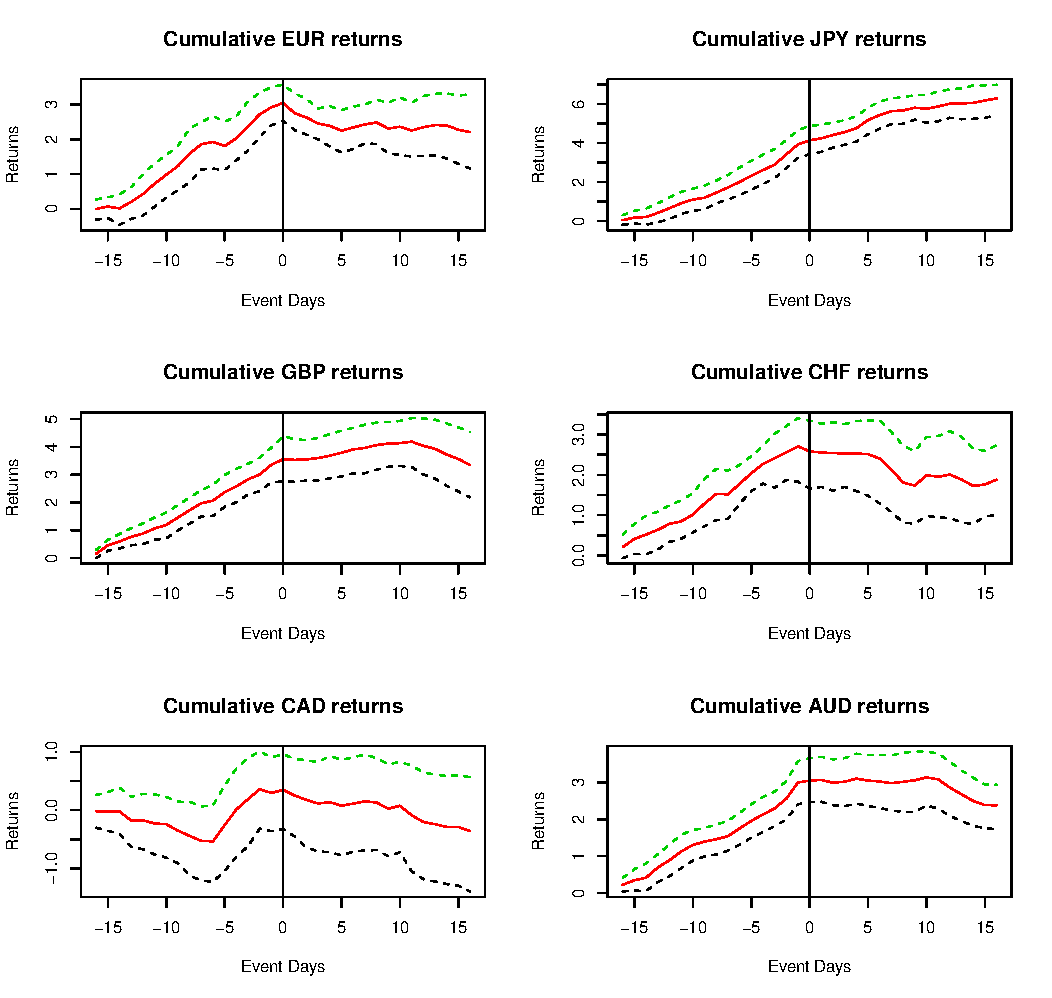
\includegraphics[scale=0.8]{RRCum16}
\end{figure}

Again, the most prominent observation is positive association between sentiment and returns.  Intuitively, this is not surprising.  However, it does suggest that foreign exchange prices are not always driven by a random walk. There is clear evidence here of serial correlation in the returns. As sentiment rises (as measured by the increase in the risk-reversal) there is a price appreciation. However, the adjustment is not instantaneous.  This is an example of the sort of trending behaviour that is common in the literature (as reported in Section \ref{secref:empiric}).  It is likely to be at least partially explained by the sort of gradual adjustment to information that was identified as being a consequence of the conservatism heuristic in Section \ref{sec:behavioural} on behavioural finance. 

\begin{figure}[h!]
\graphicspath{{../Figures/}}
\centering
\caption{Event Study:  Extreme (Low - 10th percentile) Risk Reversal Skew and 16 day event window}
\label{fig:ES2}
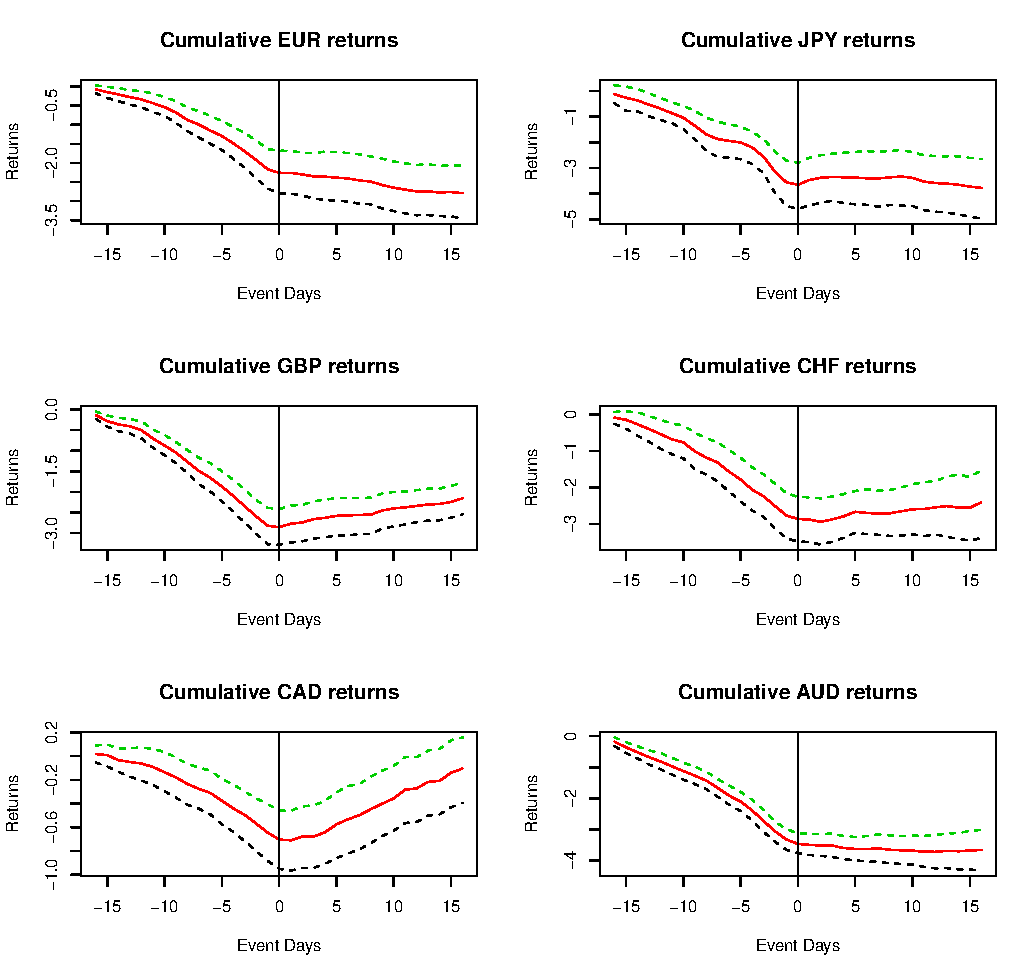
\includegraphics[scale=0.8]{RRCum16a}
\end{figure}

However, it does indicate that the evolution of exchange rates are not a random walk.  There is evidence here that prices gradually respond to information, as would be the case if decision-making is following a \emph{conservatism} heuristic or if there were institutional features.  The positive (or negative) expectations that are evident in the risk reversal skew do not seem to represent a deviation or a mis-pricing that will be reversed.  Rather they seem to be part of the price-discovery process.   

The second heuristic that was discussed in Section \ref{sec:behavioural} was representitiveness.  This was the tendency of decision-makers to focus on the immediate and to forget base probabilities.  It would suggest that investors would think too much about the new information that has driven prices towards a new equilibrium in Figures \ref{fig:ES1} and \ref{fig:ES2} not sufficient to the broad background where other currencies may be more or less attractive.  In practical terms, it suggests that there will be overshooting and that this overshooting will cause reversals when it becomes extreme.  There is little evidence here of any reversal.  After the extremes are reached, there seems more likely to be a period of consolidation or a fluctuation around the new equilibrium.  This is what would be expected if speculation were part of the process of getting information into the price. Once this has taken place, there is consolidation. 
 
\begin{landscape}
% multirow package is required.   
%pdflandscape is required to facilitate the landscape position. 
\begin{table}[ht]
\begin{threeparttable}
\caption{Event Study: Cumulative Abnormal Returns and Extreme Speculative Positions}
\begin{tabular}{llccccccccccccc}	
 % \hline
& &\multicolumn{6}{c}{S1 - Net Long per Speculators} & \multicolumn{1}{c}{} & \multicolumn{6}{c}{S2 -Net Long per Open Positions}\\
 & &\multicolumn{3}{c}{2 week} & \multicolumn{3}{c}{4 week} & \multicolumn{1}{c}{} & \multicolumn{3}{c}{2 week} & \multicolumn{3}{c}{4 week} \\ 
%\cline{4 - 10} \cline{13 - 19}
& &\multicolumn{1}{ c}{N} & \multicolumn{1}{c}{CARW} & \multicolumn{1}{c}{CARA} & \multicolumn{1}{ c}{N} & \multicolumn{1}{c}{CARW} & \multicolumn{1}{c}{CARA} & \multicolumn{1}{c}{} & 
\multicolumn{1}{ c}{N} & \multicolumn{1}{c}{CARW} & \multicolumn{1}{c}{CARA}  
& \multicolumn{1}{ c}{N} & \multicolumn{1}{c}{CARW} & \multicolumn{1}{c}{CARA}  \\   
\hline
\multirow{2}{*}{EUR} 
& Hi &  27 &  2.9415* & 1.3163* &27 & 3.8059* & 1.7341* &&27 & 1.0974* & 0.2896 &27 & 1.7667*& 0.0419  \\ 
& Lo & 27 & -2.4258* & -1.2512* & 27 &-3.9235* &-1.9254* & & 27 & -2.5122* & -1.0607* & 27 & -4.4478* & -1.9285* \\
\multirow{2}{*}{JPY}
& Hi & 43 & 1.9749* & 0.7286* & 43 & 2.8628* & 0.7909 & & 43 & 2.2463* & 1.0554* &43 & 3.7125* & 1.4443*  \\ 
& Lo & 43 & -2.2014* & -1.1312* & 43&-3.2488* & -1.5758* & &43 & -2.0605* & -0.9791* &43  & -2.6865* & -0.8318  \\
\multirow{2}{*}{GBP}
& Hi & 43 & 0.7102 & -0.2116 &43 & 1.0172* & -0.7902* & &43 & 1.2916* & 0.2370 &43 &1.6912* &0.0126  \\ 
& Lo & 43 &-0.6979* &0.2902 &43 &-1.5330* &0.1014 & &43 &-1.8993* &-0.1415 &43 &-2.8830* & -0.0768 \\
\multirow{2}{*}{CHF}
& Hi & 43 & 1.4400* & -0.0988 & 43 & 2.8665* & -0.0993 & & 43 &  2.5260* &  0.5074 & 43 & 3.6060* & 0.2158  \\ 
& Lo & 43 & -2.1816* &  -0.9770* & 43 &-3.3030* & -0.09798* & & 43 & -1.2605* & -0.3070& 43 &-0.1.6021* & 0.0670  \\
\multirow{2}{*}{CAD}
& Hi & 43 & 1.8658* & 1.0195* & 43 & 3.5298* & 1.8319* & & 43 & 2.0160* & 0.8788* &43 & 3.0995* & 0.9921*  \\ 
& Lo & 43 &-1.3238* & -0.5548* & 43 & -1.9151* & -0.7859* & & 43 & -1.2462* & -0.4505*  &43 & -1.9390*  & -0.6195*  \\
\hline
\label{tabref:SP1}
\end{tabular}
\begin{tablenotes}
\small 
\item Where Hi means extreme high in the sentient index, either S1 which is the measure of net long non-commercial (speculative) positions per number of speculators) or S2 which is the measure of net long non-commercial (speculative) positions per open interest (total outstanding open positions); high and low are above the 95th percentile or below the 5th percentile respectively; CARW is the cumulative abnormal return for the whole window, before and after the extreme event, and CARA is the cumulative abnormal return for the period after the event, which is the event day and the window; abnormal return is anything that is different from zero; the asterisk denotes significantly different from zero, where statistical significance means that more than 95\% of 1000 random bootstraps from the events are above or below zero respectively.   
\end{tablenotes}	
\end{threeparttable}  
\end{table}
\end{landscape}

Table \ref{tabref:SP1} shows the results from the event studies that were carried out using speculative positions as reported to the US regulators.  The table works in a similar way to Table \ref{tabref:RR1}.  The first column is the exchange rate, defined as units per US dollar.  The table is then split into two parts.  The first part uses the measure S1 which is the net non-commercial (speculative) positions relative to total non-commercial (speculative) positions; the second is S2 as the net non-commercial position relative to open interest or the total outstanding open positions.  Therefore, the first captures the balance of speculative positions while the second captures the balance of speculative positions relative to the whole market.  If speculators become more prevalent or dominant in the market, this will show up in S2 but not S1.  S1 is more sensitive to changes in sentiment and more volatile.\footnote{When the same data are used in the model for international capital flows in ref, it is found that S1 tends to provide a better fit for the module of capital flow and the real trade weighted index.} Each of these sections is broken into the results for a 2 week window and a 4 week window.  Each of these has the same pattern.   There is a row for extreme high and extreme low which represents extreme long positions or extreme short positions; the first  column identifies the number of cases; CARW is the cumulative abnormal return for the whole event window; CARA is the cumulative abnormal return for the period after the event to the end of the window.     

\begin{figure}[h!]
\graphicspath{{../Figures/}}
\centering
\caption{Event Study:  Extreme (95th percentile), Non-commercial net per OI (S2), 6 week event window}
\label{fig:ES3}
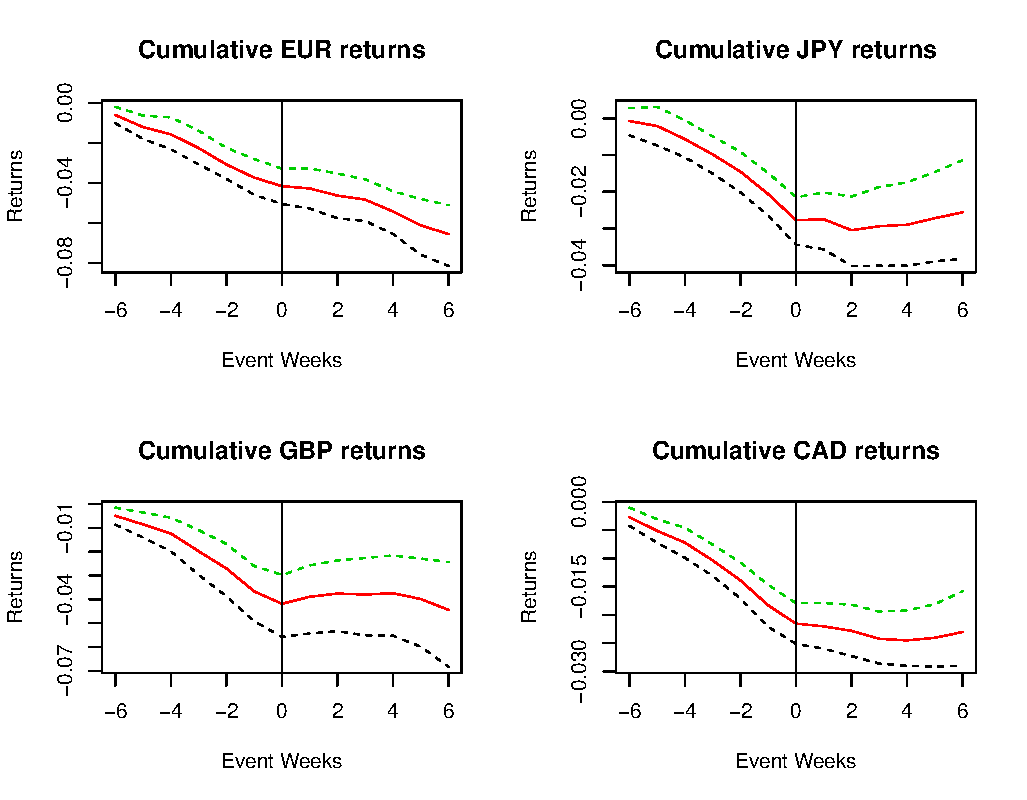
\includegraphics[scale=0.8]{FPCum6w}
\end{figure}

Once again, there is a very strong association between returns and the movement of speculators.  For the 4-day window and the S1 and S2 measures, every one of the currencies studied, high and low, had a mean cumulative return for the whole of the event window that was in the same direction as sentiment.  When re-sampled a thousand times, more than ninety five percent of the means calculated were greater than zero in all cases but one (GBP).  Once again there is evidence here of momentum and of speculator positions following the movement of prices.    

However, there is little evidence that these speculators are driving prices to extremes with their extreme behaviour.  Sixty percent of the S1 cases still show a significant abnormal return in the direction of the extreme 4 weeks after the extreme has been reached; only thirty percent of the cases show a reversal and in only one of those do ninety five percent of the re-sampled means remain above zero.  For S2 it is even more extreme, with ninety percent of the cases showing a continuation and forty percent of them being significant.  Again the evidence is consistent with the gradual adjustment of prices to information. 

\begin{figure}[h!]
\graphicspath{{../Figures/}}
\centering
\caption{Event Study:  Extreme (90th percentile), Non-commercial net long (S1), 6 week window}
\label{fig:ES4}
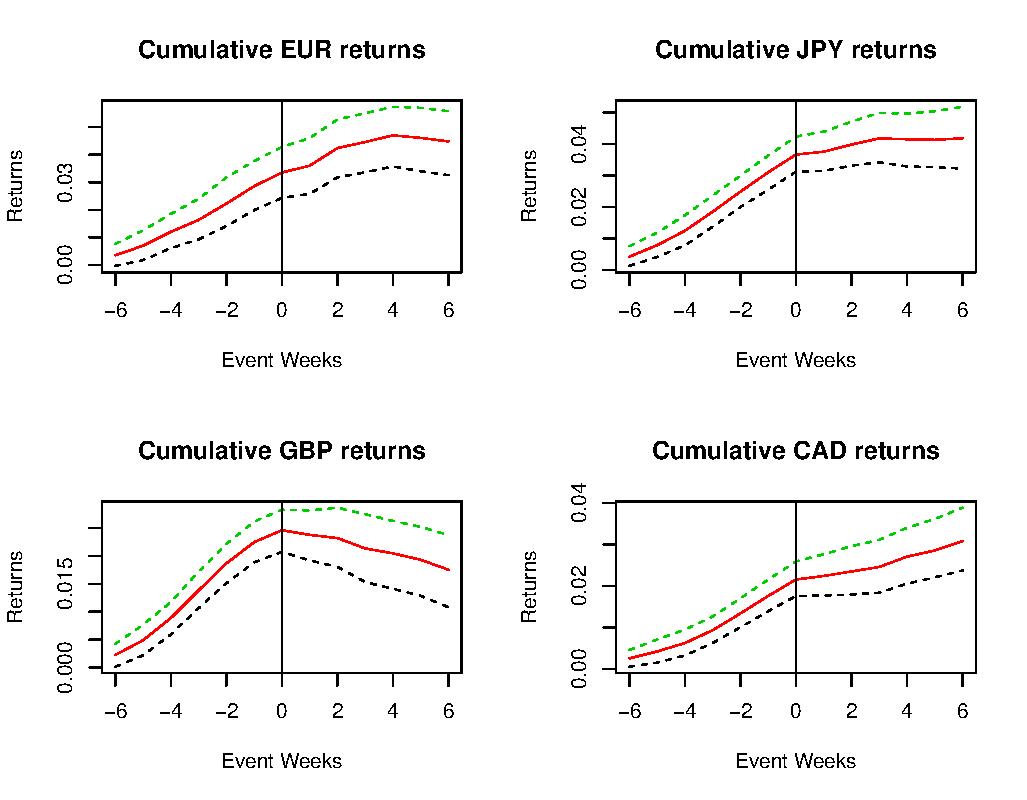
\includegraphics[scale=0.8]{FPCum6wa}
\end{figure}

The R code for all the event window figures is available in Appendix \ref{AppendixB} Section \ref{Asecref:event}.  This merely takes the data that was used to construct Tables \ref{tabref:RR1} and \ref{tabref:SP1} and puts it in graphical form.  The event windows are stretched to give a clear view of the evolution of exchange rates  around the event.  Confidence intervals are added.  Once event objects FX.exc have been created, parameter for exchange rate, extreme measure, quantile, window length and the high or low indicator can be changed for alternative assessments of speculative extremes. Adjustments to these parameters show that these results are not a function of the choices presented in the main text.  They are robust to alternative specifications. 

Figure \ref{fig:ES3} shows the performance of the cumulative abnormal returns around a six week event window where the event is the net low (short) speculative positions relative to total activity (open interest) at or below the ($5\%)$ level.  This means that the speculators are inclined to be short the non-domestic (US dollar) currency.  While the Euro continues to move lower after the extreme short positions, the other major currencies seem to reveal a period of consolidation that is consistent with the settlement around an equilibrium after a period where information is being absorbed.  The contrast between the Euro and the other currencies may be associated with the fact that there is a smaller dataset for the Euro due to its more limited lifespan.  Figure \ref{fig:ES4} shows the abnormal returns around extreme high (90th percentile and long position).  There is some tentative evidence of continuation for speculative positions in the Canadian dollar and signs of reversal for UK sterling.  However, the Euro and the Japanese yen move sideways after the event.  There is no clear pattern after the extreme and therefore no information.  

\section{Speculation and foreign exchange returns}
This chapter has sought to measure speculation and to use this measure to discover more about the relationship between speculation, information and asset prices.  The measurement of speculation takes two forms:  a measurement of the intensity of belief with the risk-reversal skew, and a measurement of speculative positions.  Neither of these is ideal, in the sense of being a random sample from a population.  However, the option prices reveal the intensity of feeling through the weight of money in a speculative part (options) of a speculative market (foreign exchange).  The commitment of traders report records only speculators in the US futures market.  However, this is an important market, there is no reason to believe that US or speculators in the futures market are systematically different from those in the rest of the world and presumably if there were a major difference there would be an arbitrage opportunity between the two markets.  

 there is strong evidence that speculation affects prices and that this effect is gradual rather than instantaneous.  This suggests a market inefficiency that would reward momentum-based trading.  It is no wonder therefore that \citep{TaylorTechnical}, reporting a survey conducted by the Bank of England, found that of the Chief foreign exchange dealers contacted in London in November 1988, 90\% of them attached some weight to \emph{technical analysis}, a method that is fundamentally based on finding trends in asset prices.  The survey found that the importance of technical analysis became greater at shorter horizons.  This has not disappeared.  The importance of momentum trading and technical analysis has not waned with time.  Neely and Wller  show that gains from technical trading rules still generate excess returns and attribute this to behavioural biases \citep{NeelyWeller}. It seems that speculation forms part of the process of price discovery, but this process is not instantaneous as would be expected in the purest form of the EMH.  

The notion that speculation is at least partially informed is supported by the fact that there is little evidence from the event studies conducted here that speculation causes overshooting or bubbles.  When speculation is extreme, whether measured by intensity of belief or weight of speculative positions, future returns are as likely to be positive as negative.  There is no informational content as there would be if speculation was pure noise.  In the simulation of the De Long model, extremes are more likely to be followed by reversals.  In the foreign exchange market, that is not the case.  There are some large price crashes in the dataset, as shown by the descriptive statistics of the returns. For example  in Table \ref{tabref:DS1} it is seen that on one day there is a 10.65\% appreciation of the Japanese yen and Table \ref{tabref:DS2} shows a week when the Canadian dollar falls by 10\%.  However, the measures of speculative sentiment or the weight of speculation are not particularly high in either of these cases.  Indeed, an analysis of the top 1\% of positive and negative foreign exchange returns in the dataset reveals that sentiment and positions for this group were very close to the average of the whole set.  This would be consistent with a model where extreme price movement was a function of new information rather than the structure of existing positions.    
%expand.  Could put data in appendix.  
 
The evidence here, that speculation is associated with serial correlation in the returns but cannot be used in a systematic way to determine reversals, has important implications for speculative activity.  It means that the largest returns will be to those that identify the trend at the earliest opportunity.  This means that speculators must be prepared to act as swiftly as possible, probably when there is a high level of uncertainty and a lack of information and where any scrap of additional news is highly valued.   The risk that actions by other speculators, most notable by their effect on price, will be construed to contain information exacerbates the likelihood of feedback effects.  The need to be able to take action before others has reached the most extreme form in the activity of \emph{high frequency trading} (HFT), where decision times are measured in nanoseconds and there is advantage in gaining spacial proximity to exchanges.  HFT is all about getting  a larger share of the inefficiency in pricing information by trading or investing closer to where the information is released.  

These findings have implications for speculators, economic modellers and policy makers.  Speculators may jump on the trend, but they do not know by looking at how popular that trend is when to get off.  They need other signs to tell them that the trend has reached its conclusion or equilibrium has been achieved.  For the modellers, there is confirmation of the need  for feedback effects and evidence that reversals cannot be systematically identified from high levels of speculative positions.  It may suggest another trigger for bursting bubbles; it may, for example, suggest that this reversal has to be modelled as stochastic element or pure shock. For policy makers, there is no escape from the requirement to look at economic fundamentals when deciding whether bubbles are building in asset markets.  The presence of speculators is no guarantee that there is excess.  The speculators may be just part of the adjustment to new information.   However, the combination of high level of speculation and divergence from fundamentals is likely to create the greatest risk. 

\bibliography{myrefs}



\end{document}